\documentclass{ltxdockit}
\usepackage{btxdockit}
\usepackage[british]{babel}
\usepackage[strict=true,autostyle=true]{csquotes}
\usepackage{ifthen}
\usepackage{fontspec}
\usepackage{tikz}
\usepackage{graphicx}
\usepackage{booktabs}
\usepackage{fixfoot}
\usepackage{xcolor}
\usepackage{listings}
\usepackage{metalogo}
\usepackage{colortbl}

\usepackage[retainmissing]{MnSymbol}
\setmainfont[Ligatures=TeX]{CMU Serif}
\setsansfont[Ligatures=TeX]{CMU Sans Serif}
\setmonofont{CMU Typewriter Text}

\def\BibLaTeX{\textsc{Bib}\latex}
\def\BibTeX{\textsc{Bib}\kern-.08em \TeX}

\renewcommand{\labelitemii}{$\circ$}
\newcommand*{\biber}{Biber\xspace}
\newcommand*{\biblatex}{Biblatex\xspace}
\MakeAutoQuote{«}{»}

\gdef\biberversion{2.14}    % BIBER VERSION
\gdef\biblatexversion{3.14}   % BIBLATEX VERSION

% colour for tables
\definecolor{Gray}{gray}{0.85}

\newcolumntype{a}{>{\columncolor{Gray}}l}

% Set up tikz things
\usetikzlibrary{shapes.geometric}
\usetikzlibrary{arrows}
\usetikzlibrary{fit}
\usetikzlibrary{calc}
\tikzstyle{file} = [rectangle, black, very thick, draw=blue, fill=blue!20,
                    minimum width=6em, minimum height=3em, align=center]
\tikzstyle{funit} = [rectangle, rounded corners=1ex, black, very thick,
                     shape border rotate=-90, draw=green, fill=green!20,
                     minimum size=3em, align=center]

% colours for the .dot examples
\xdefinecolor{centry}{HTML}{A0D0FF}
\xdefinecolor{ncentry}{HTML}{DEEFFF}
\xdefinecolor{doentry}{HTML}{FDFFD9}
\xdefinecolor{section}{HTML}{FCE3FA}
\xdefinecolor{set}{HTML}{E3DADC}
\xdefinecolor{related}{HTML}{AD1741}
\xdefinecolor{clone}{HTML}{AD1741}
\xdefinecolor{crossref}{HTML}{7D7879}
\xdefinecolor{xref}{HTML}{7D7879}
\xdefinecolor{xdata}{HTML}{2CA314}

\DeclareFixedFootnote{\tpb}{Binary maintained by third party. See README in
  binary download directory for this platform for support/contact
  details. Usually, the binary maintainer is also the binary build
  provider for \TeX Live.}

\titlepage{%
  title={biber},
  subtitle={A backend bibliography processor for biblatex},
  url={http://biblatex-biber.sourceforge.net},
  author={Philip Kime, François Charette},
  email={Philip@kime.org.uk},
  revision={biber \biberversion\ (biblatex \biblatexversion)},
  date={\today}}

\hypersetup{%
  pdftitle={biber},
  pdfsubject={A backend bibliography processor for biblatex},
  pdfauthor={Philip Kime},
  pdfkeywords={biblatex, bibliography}}


% Control list spacing
\usepackage{enumitem}
\setdescription{noitemsep}
\setenumerate{noitemsep}
\setitemize{noitemsep}

\def\biberex#1{\hbox{\hspace{-4em}\texttt{\small \detokenize{#1}}}}

\begin{document}
\definecolor{grey}{rgb}{0.7,0.7,0.7}
\printtitlepage
\tableofcontents

\section{Important Changes}\label{special}

Please see the \verb+Changes+ file which accompanies \biber\ for the
details on changes in each version. This section is just for important
things like incompatible changes which users should be aware of.

\minisec{2.13}
In tool mode (\opt{--tool}), \biber now allows datamodel configuration in
a user configuration file to add to or override the default datamodel
contained in the main \file{biber-tool.conf} file. Previously it was
necessary to copy the entire default data model into a user configuration
file and then alter it.

\minisec{2.6}
When outputting \bibtex\ data in tool mode (\opt{--tool}), \biber now
follows a full internal processing chain involving the data model. In
previous versions, \bibtex output would just output the raw
\bibtex input data, only allowing for some re-formatting options and
therefore no tool mode conversions from other formats into \bibtex format
were possible. This change has some normalisation consequences:

\begin{itemize}
\item Dates are normalised into \bibfield{DATE} fields. Legacy
  \bibfield{YEAR} fields are never output in \bibtex format data output.
\item Fields which are not defined in the data model described in the
  default \file{biber-tool.conf} are ignored and are neither read nor
  output. If custom fields are required, they should be defined in the data
  model by using a custom tool mode config file (see below). If you would
  like to have ignored fields reported on, use the
  \opt{--validate-datamodel} option.
\end{itemize}

\minisec{1.9}
\biber no longer checks the environment for locales to use for sorting. This
was always rather against the spirit of \tex since it means that the same
document might look different when compiled by different people. However,
\biblatex now passes Babel/Polyglossia language identifiers (or real locale
identifiers if you prefer) in the \file{.bcf} and \biber can use these to
set the sorting locale globally or on a per-sortscheme basis. This is better
than using environment variables since Babel/Polyglossia are more \latex
relevant language environments anyway.

\minisec{1.8}
Various option name changes. Old names are retained for backwards
compatibility. See the output of the \opt{--help} option.

\minisec{1.0}
The \opt{--validate-structure} option is now called \opt{--validate-datamodel}

\minisec{0.9.9}
The output format option \opt{--graph} has been moved to a
new option \opt{--output-format}. The option \opt{--graph} should now be
specified as \opt{--output-format=dot} and the \linebreak\opt{--dot-include} option
should be used to specify the elements to include in the DOT output. For
example:

\begin{verbatim}
  biber --graph=section,field <file>
\end{verbatim}

\noindent is now:

\begin{verbatim}
  biber --output-format=dot --dot-include=section,field <file>
\end{verbatim}

\minisec{1.8}
\textcolor{red}{Several option names have changed}. Several options have
changed names to facilitate better semantic classification of options. The
previous names are supported as legacy aliases. See the \opt{--help}
output of the \biber command.

\minisec{0.9.8}
\textcolor{red}{The \opt{sourcemap} option syntax has changed}.The syntax
was too confusing. It is now simplified and more powerful. It is uses a
sequential processing model to apply mappings to an entry. See section
\ref{ref:map}.

\minisec{0.9.7}
\textcolor{red}{The user config file has a completely new format}.The
  reason for this is that the older \verb+Config::General+ format
  could not be extended to deal with more sophisticated features like
  per-datasource restrictions. An XML format is much better and in
  fact easier to understand. The old format of the \opt{map} option
  (now called \opt{sourcemap}) was rather confusing because
  of limitations in the old config file format. Please see section
  \ref{ref:map} and convert your config files to the new format.

\minisec{0.9.6}
\textcolor{red}{Matching of citation keys and datasource entry keys is now
  \emph{case-sensitive}}. This is to enforce consistency across the entire
Bib\latex\ and \biber\ processing chain. All of the usual referencing
mechanisms in \latex\ are case-sensitive and so is the matching in
Bib\latex\ of citations to entries in the \texttt{.bbl} file generated by
\biber. It is inconsistent and messy to enforce case-insensitivity in only
\biber's matching of citations keys to datasource entry keys. If \biber\
detects what looks like a case mismatch between citation keys, it will warn
you.

\noindent \textcolor{red}{Summary of warnings/errors is now a new format}.
When \biber\ finishes writing the \verb+.bbl+, it gives a summary
count of errors/warnings. It used to do this in the same format as
Bib\TeX, for compatibility. Now it uses a more consistent and easier
to parse format which matches all other \biber\ messages. Please note
if you need to support \biber\ in an external tool. I have updated the
notes on AUC\TeX\ support below to reflect this.

\section{Introduction}\label{int}

\subsection{About}

\biber\ is conceptually a \BibTeX\ replacement for
\biblatex. It is written in Perl with the aim of providing a
customised and sophisticated data preparation backend for \biblatex.
You do \emph{not} need to install Perl to use \biber---binaries
are provided for many operating systems via the main \TeX\
distributions (\TeX Live, Mac\TeX, MiK\TeX) and also via download from SourceForge.
Functionally, \biber\ offers a superset of \BibTeX's capabilities but is
tightly coupled with \biblatex\ and cannot be used as a stand-alone tool
with standard \verb+.bst+ styles. \biber's primary role is to support
\biblatex\ by performing the following tasks:

\begin{itemize}
\item Parsing data from datasources
\item Processing cross-references, entry sets, related entries
\item Generating data for name, name list and name/year disambiguation
\item Structural validation according to \biblatex\ data model
\item Sorting reference lists
\item Outputting data to a \verb+.bbl+ for \biblatex\ to consume
\end{itemize}

\biber\ also has the ability to output different formats than \file{.bbl}
and can, for example, output a new \bibtex\ file which contains only
cited entries from the datasources (using the \opt{--output-format=bibtex}
option). There is also a «<tool» mode which operates on datasources instead
of individual documents, allowing you to transform, convert, reformat and
generally change the contents of a datasource (see \ref{ref:tool}).

\subsection{Requirements}\label{ref:req}

\biber\ is distributed primarily as a stand-alone binary and is
included in \TeX Live, Mac\TeX\ and MiK\TeX. If you are using any of these
distributions, you do not need any additional software installed to use
\biber. You do \emph{not} need a Perl installation at all to use
the binary distribution of \biber\footnote{If you prefer, you can run
\biber\ as a normal Perl program and doing this \emph{does} require
you to have a Perl interpreter installed. See section \ref{binaries}.}.

\biber's git repository and bug/feature tracker is on
github\footnote{\url{https://github.com/plk/biber}}. \biber's documentation,
binary downloads and supporting files are on
SourceForge\footnote{\url{http://sourceforge.net/projects/biblatex-biber/}}
\biber\ is included into \TeX Live, the binaries coming from SourceForge.

\subsection{Compatibility Matrix}

\biber\ versions are closely coupled with \biblatex\ versions. You
need to have the right combination of the two. \biber\ will warn you
during processing if it encounters information which comes from a
\biblatex\ version which is incompatible. Table \ref{tab:compat} shows a
compatibility matrix for the recent versions.

\begin{table}
\begin{center}
\small
\begin{tabular}{lllll}
\toprule
\biber\ version & \biblatex\ version\\
\midrule
2.13 & 3.13\\
2.12 & 3.12\\
2.11 & 3.11\\
2.10 & 3.10\\
2.9 & 3.9\\
2.8 & 3.8\\
2.7 & 3.7\\
2.6 & 3.5, 3.6\\
2.5 & 3.4\\
2.4 & 3.3\\
2.3 & 3.2\\
2.2 & 3.1\\
2.1 & 3.0\\
2.0 & 3.0\\
1.9 & 2.9\\
1.8 & 2.8x\\
1.7 & 2.7\\
1.6 & 2.6\\
1.5 & 2.5\\
1.4 & 2.4\\
1.3 & 2.3\\
1.2 & 2.1, 2.2\\
1.1 & 2.1\\
1.0 & 2.0\\
0.9.9 & 1.7x\\
0.9.8 & 1.7x\\
0.9.7 & 1.7x\\
0.9.6 & 1.7x\\
0.9.5 & 1.6x\\
0.9.4 & 1.5x\\
0.9.3 & 1.5x\\
0.9.2 & 1.4x\\
0.9.1 & 1.4x\\
0.9 & 1.4x\\
\bottomrule
\end{tabular}
\end{center}
\caption{\biber/\biblatex\ compatibility matrix}
\label{tab:compat}
\end{table}

\subsection{License}

\biber\ is released under the free software Artistic License 2.0\footnote{\url{http://www.opensource.org/licenses/artistic-license-2.0.php}}

\subsection{History}

\BibTeX\ has been the default (only \ldots) integrated choice for
bibliography processing in \TeX\ for a long time. It has well known
limitations which stem from its data format, data model and lack of Unicode
support\footnote{In fact, there is now a Unicode version}. The
\verb+.bst+ language for writing bibliography styles is painful to learn
and use. It is not a general programming language and this makes it really
very hard to do sophisticated automated processing of bibliographies.

\biblatex\ was a major advance for \latex\ users as it moved much
of the bibliography processing into \latex\ macros. However,
\biblatex\ still used \BibTeX\ as a sorting engine for the
bibliography and also to generate various labels for
entries. \BibTeX's capabilities even for this reduced set of
tasks was still quite restricted due to the lack of Unicode support and
the more and more complex programming issues involved in label
preparation and file encoding.

\biber\ was designed specifically for \biblatex\ in order to
provide a powerful backend engine which could deal with any required
tasks to do with \verb+.bbl+ preparation. Its main features are:

\begin{itemize}
\item Deals with the full range of UTF-8
\item Sorts in a completely customisable manner using, when available,
  CLDR collation tailoring
\item Allows for per-entrytype options
\item Automatically encodes the \verb+.bbl+ into any supported encoding
  format\footnote{«Supported» here means encodings supported by the
    Perl \texttt{Encode} module}
\item Processes all bibliography sections in one pass of the tool
\item Output to GraphViz instead of \verb+.bbl+ in order to help visualise
  complex bibliographies with many crossrefs etc. (see section \ref{ref:vis})
\item Handles UTF-8 citekeys and filenames (given a suitable fully
  UTF-8 compliant \TeX\ engine)
\item Creates entry sets dynamically and allows easily defined static entry sets,
  all processed in one pass
\item «Syntactic» inheritance via new \bibtype{XDATA} entrytype and
  field. This can be thought of as a field-based generalisation of the
  \BibTeX\ \bibtype{STRING} functionality (which is also supported).
\item «Semantic» inheritance via a generalisation of the \BibTeX\
  crossreference mechanism. This is highly customisable by the
  user---it is possible to choose which fields to inherit for which
  entrytypes and to inherit fields under different names etc. Nested
  crossreferences are also supported.
\item Handles complex auto-expansion and contraction of names and
  namelists (See section 4.11.4 of the \biblatex\ manual for an excellent
  explanation with examples, this is quite an impressive feature \ldots)
\item Extensible modular datasource architecture for ease of adding
  more datasource types
\item Support for remote datasources
\item User-definable mapping and suppression of fields and entrytypes in
  datasources. You can use this to, for example, ignore all
  \bibfield{ABSTRACT} fields completely. See section \ref{ref:map}
\item Support for related entries, to enable generic treatment of things
  like «translated as», «reprinted as», «reprint of»
  etc.
\item Customisable labels
\item Multiple bibliography lists in the same section with different
  sorting and filtering
\item No more restriction to a static data model of specific fields and
  entrytypes
\item Structural validation of the data against the data model with a
  customisable validation model
\item Tool mode for operations on datasources directly
\end{itemize}

\noindent Figure \ref{fig:overview} shows the main functional units of
processing in \biber. The most difficult tasks which \biber\
performs are the processing of \biblatex's \opt{uniquename} and
\opt{uniquelist} options\footnote{A rather tricky unbounded loop but with
  a guaranteed eventual stable exit state.}, the sorting of
lists\footnote{This is multi-field ST sort with an embedded cache for
 performance.} and the initial data parse and remap into an
internal data model. \biber\ is getting on for around 20,000 lines of
mostly OO Perl and relies on certain splendid Perl modules
such as \verb+Unicode::Collate+, \verb+Text::BibTeX+ and
\verb+XML::LibXML+.

\begin{figure}[!htpb]
  \centering\small
  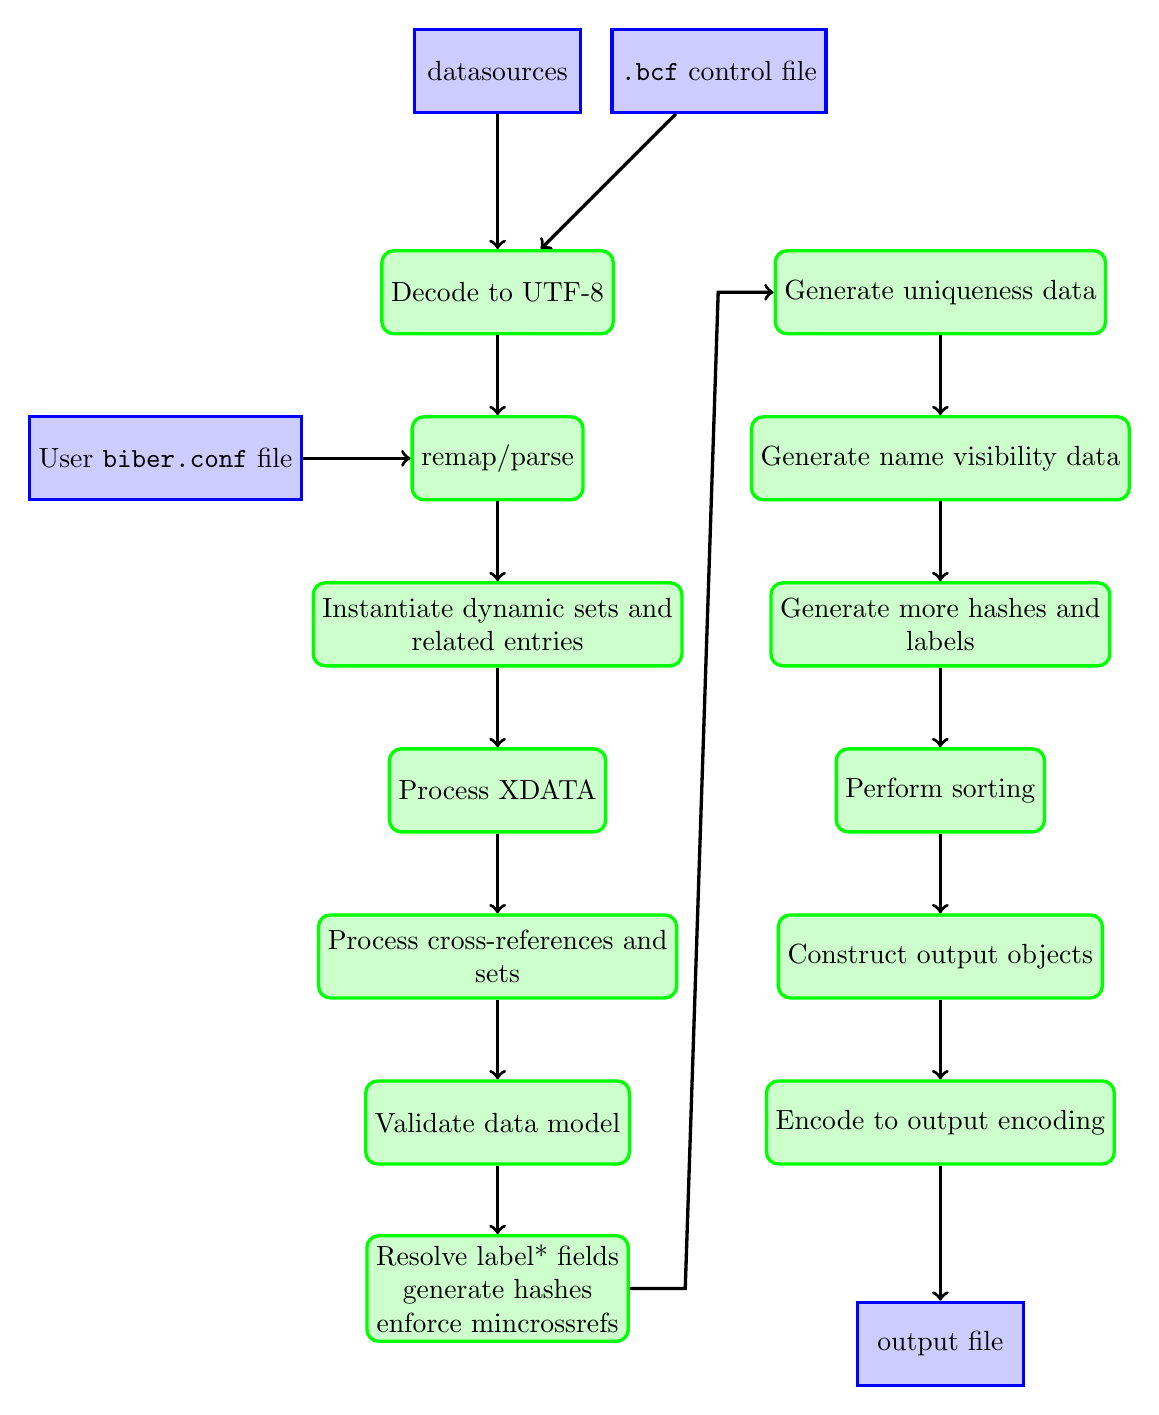
\begin{tikzpicture}
    \node[file] (dsfiles) {datasources};
    \node[file] (bcf) [right of=dsfiles,node distance=8em] {\texttt{.bcf} control file};
    \node[funit] (decode) [below of=dsfiles,node distance=8em] {Decode to UTF-8} edge [<-,very thick] (dsfiles) edge [<-,very thick] (bcf);
    \node[funit] (mapp) [below of=decode,node distance=6em] {remap/parse} edge [<-,very thick] (decode);
    \node[file] (config) [left of=mapp,node distance=12em] {User \texttt{biber.conf} file} edge [->,very thick] (mapp);
    \node[funit] (dyn) [below of=mapp,node distance=6em] {Instantiate dynamic sets and\\related entries} edge [<-,very thick] (mapp);
    \node[funit] (xdata) [below of=dyn,node distance=6em] {Process XDATA} edge [<-,very thick] (dyn);
    \node[funit] (crossrefs) [below of=xdata,node distance=6em] {Process cross-references and\\sets} edge [<-,very thick] (xdata);
    \node[funit] (validate) [below of=crossrefs,node distance=6em] {Validate data model} edge [<-,very thick] (crossrefs);
    \node[funit] (pre) [below of=validate,node distance=6em] {Resolve label* fields\\generate hashes\\enforce mincrossrefs} edge [<-,very thick] (validate);
    \node[funit] (unique) [right of=decode,node distance=16em] {Generate uniqueness data};
    \draw[->,very thick] (pre.east) -- ($ (pre.east) + (2em,0) $) -- ($ (unique.west) - (2em,0) $) -- (unique.west);
    \node[funit] (visible) [below of=unique,node distance=6em] {Generate name visibility data} edge [<-,very thick] (unique);
    \node[funit] (post) [below of=visible,node distance=6em] {Generate more hashes and\\labels} edge [<-,very thick] (visible);
    \node[funit] (sort) [below of=post,node distance=6em] {Perform sorting} edge [<-,very thick] (post);
    \node[funit] (output) [below of=sort,node distance=6em] {Construct output objects} edge [<-,very thick] (sort);
    \node[funit] (encode) [below of=output,node distance=6em] {Encode to output encoding} edge [<-,very thick] (output);
    \node[file] (bbl) [below of=encode,node distance=8em] {output file} edge [<-,very thick] (encode);
  \end{tikzpicture}
  \caption{Overview of \biber's main functional units}
  \label{fig:overview}
\end{figure}

It may be useful to know something about the different routes a datasource
entry can take as it passes through \biber.

\begin{enumerate}
\item\label{list:cited} All cited entries which are subsequently found in a
  datasource are instantiated in the internal \biber\ data model.
\item Some uncited entries on which cited entries depend are
  instantiated in the internal \biber\ data model:
  \begin{itemize}
  \item Entries with entrytype \bibtype{XDATA} which are referenced from cited
    entries.
  \item Entries mentioned in the \bibfield{CROSSREF} or
    \bibfield{XREF} field of a cited entry (unless they are also cited
    themselves in which case they are already instantiated as per item
    \ref{list:cited} above).
      \item Clones of entries mentioned as a «related» entry of a cited
        entry.
      \item Members of sets, either explicit \bibtype{SET} entrytype entries or
        dynamic sets.
  \end{itemize}
\item Some uncited but instantiated entries are promoted to cited
  status so that they make it into the output:
  \begin{itemize}
  \item Entries instantiated by being members of a set.
  \item Entries instantiated by being mentioned as a \bibfield{CROSSREF} are
    promoted to cited status if \bibfield{CROSSREF}'ed or \bibfield{XREF}'ed at
    least \opt{mincrosref} times.
  \item Clones of entries mentioned as a «related» entry of a cited entry.
  \end{itemize}
\item Some of these auto-cited entries have the «dataonly» option set on
  them so that \biblatex\ will only use them for data and will not output
  them to the bibliography:
  \begin{itemize}
  \item Clones of entries mentioned as a «related» entry of a cited entry.
  \end{itemize}
\end{enumerate}

\subsection{Performance}

\biber\ can't really be compared with \BibTeX\ in any meaningful
way performance-wise. \biber\ is written in Perl and does a
\emph{great} deal more than \BibTeX\ which is written in C. One of
\biber's test cases is a 2150 entry, 15,000 line \verb+.bib+ file
which references a 630 entry macros file with a resulting 160 or so page (A4)
formatted bibliography. This takes \biber\ just under 30 seconds to process on
a reasonable computer. This is perfectly acceptable, especially for a
batch program.

\subsection{Acknowledgements}

François Charette originally wrote a first modest version of \biber. Philip Kime joined in
the development in 2009 and is largely responsible for making it what it is today. 

\section{Use}

Firstly, please note that \biber\ will \emph{not} attempt to sanitise
the content of \BibTeX\ datasources. That is, don't expect it to
auto-escape any \TeX\ special characters like «\verb+&+» or «\verb+%+» which
it finds in, for example, your \bibfield{TITLE} fields. It used to do this in
earlier versions in some cases but as of version 0.9, it doesn't because
it's fraught with problems and leads to inconsistent expectations and
behaviour between different datasource types. In your \BibTeX\ data
sources, please make sure your entries are legal \TeX\ code.

Running \opt{biber --help} will display all options and description of
each and is the primary source of usage information. \biber\
returns an exit code of 0 on success or 2 if there was an error.

Most \biber\ options can be specified in long or short format. When
mentioning options below, they are referred to as
«\opt{long form|short form}» when an option has both a long and short
form. As usual with such options, when the option requires an argument, the
long form is followed by an equals sign «\verb+=+» and then the argument,
the short form is followed by a space and then the argument. For example,
the \opt{--configfile|-g} option can be given in two ways:

\begin{verbatim}
biber --configfile=somefile.conf
biber -g somefile.conf
\end{verbatim}

With the \opt{backend=biber} option, \biblatex\ switches its backend
interface and passes all options and information relevant to \biber's
operation in a control file with extension \verb+.bcf+\footnote{\biblatex\ Control
  File}. This is conceptually equivalent to the \verb+.aux+ file which
\latex\ uses to pass information to \BibTeX. The \verb+.bcf+ file is
XML and contains many options and settings which configure how \biber\
is to process the bibliography and generate the \verb+.bbl+ file.

The usual way to call \biber\ is simply with the \verb+.bcf+ file
as the only argument. \biblatex\ always writes the control file with
a \verb+.bcf+ extension. Specifying the «\verb+.bcf+» extension to
\biber\ is optional. Assuming a control file called
\verb+test.bcf+, the following two commands are equivalent:

\begin{verbatim}
biber test.bcf
biber test
\end{verbatim}

\noindent Figure \ref{fig:biber-mdf} is a graphical overview of the data flow for
data model information. See Figure \ref{fig:overview} for a more complete
overview of \biber's processing steps.

\begin{figure}[!htpb]
  \centering\small
  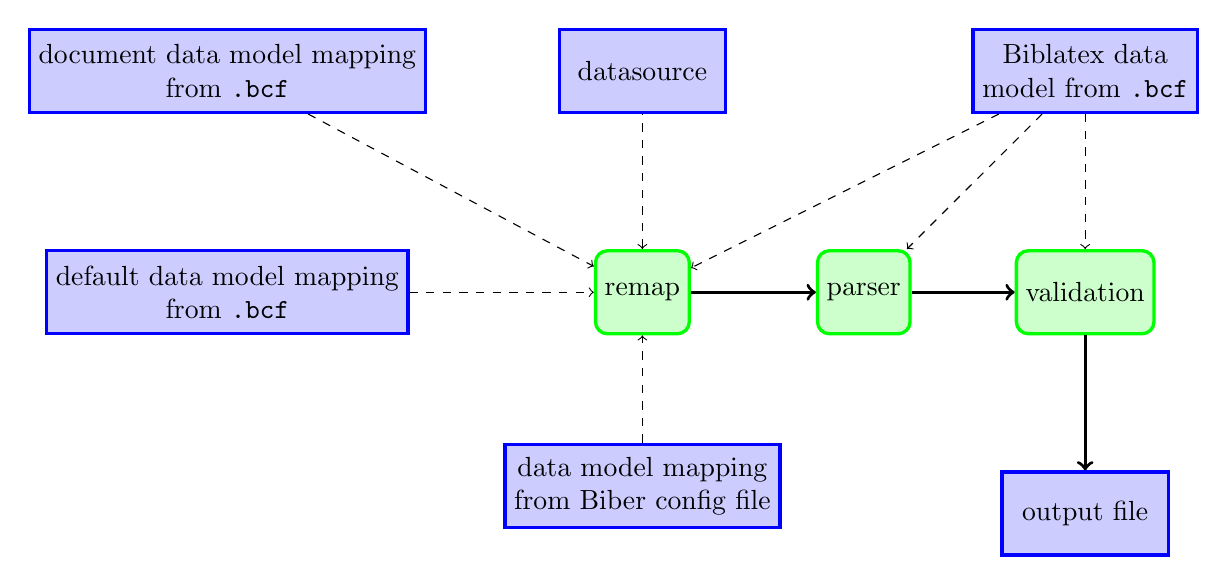
\begin{tikzpicture}
    \node[file] (dsfile) {datasource};
    \node[funit] (remap) [below of=dsfile, node distance=8em] {remap} edge [<-,dashed] (dsfile);
    \node[file] (docremap) [left of=dsfile, node distance=15em] {document data model mapping\\from \texttt{.bcf}} edge [->,dashed] (remap);
    \node[file] (defaultremap) [left of=remap, node distance=15em] {default data model mapping\\from \texttt{.bcf}} edge [->,dashed] (remap);
    \node[file] (conf) [below of=remap,  node distance=7em] {data model mapping\\from \biber\ config file} edge [->,dashed] (remap);
    \node[funit] (parser) [right of=remap, node distance=8em] {parser} edge [<-,very thick] (remap);
    \node[funit] (validation) [right of=parser, node distance=8em] {validation} edge [<-,very thick] (parser);
    \node[file] (hard) [above of=validation, node distance=8em]
    {\biblatex\ data\\model from \texttt{.bcf}} edge [->,dashed]
    (parser) edge [->,dashed] (remap) edge [->,dashed] (validation);
    \node[file] (bbl) [below of=validation, node distance=8em] {output file} edge [<-,very thick] (validation);
  \end{tikzpicture}
  \caption{Model data flow in \biber}
  \label{fig:biber-mdf}
\end{figure}
\bigskip
\subsection{Options and config file}\label{conffile}
\biblatex\ options which \biber\ needs to know about are passed
via the \verb+.bcf+ file. See Table \ref{tab:bltxopts} for the \biblatex\
options which \biber\ uses and also for the scopes which are supported
for each option. \biber\ also has its own options which are set using
the following resource chain, given in decreasing precedence order:\\[2ex]

\begin{table}
\begin{center}
\small
\begin{tabular}{lllll}
\toprule
\biblatex\ option & Global & Per-type & Per-entry\\
\midrule
alphaothers        & \checkmark & \checkmark &  \\
dataonly           &   & \checkmark  & \checkmark\\
inheritance        & \checkmark &   &  \\
labelalpha         & \checkmark & \checkmark &  \\
labelalphatemplate & \checkmark & \checkmark &  \\
labeldate          & \checkmark & \checkmark &  \\
labeldatespec      & \checkmark & \checkmark &  \\
labelnamespec      & \checkmark & \checkmark &  \\
labelnumber        & \checkmark & \checkmark &  \\
labeltitle         & \checkmark & \checkmark &  \\
labeltitleyear     & \checkmark & \checkmark &  \\
maxalphanames      & \checkmark & \checkmark & \checkmark\\
maxbibnames        & \checkmark & \checkmark & \checkmark\\
maxcitenames       & \checkmark & \checkmark & \checkmark\\
maxitems           & \checkmark & \checkmark & \checkmark\\
minalphanames      & \checkmark & \checkmark & \checkmark\\
minbibnames        & \checkmark & \checkmark & \checkmark\\
mincitenames       & \checkmark & \checkmark & \checkmark\\
minitems           & \checkmark & \checkmark & \checkmark\\
presort            & \checkmark & \checkmark & \checkmark\\
singletitle        & \checkmark & \checkmark &  \\
skipbib            &   & \checkmark & \checkmark\\
skiplab            &   & \checkmark & \checkmark\\
skiplos            &   & \checkmark & \checkmark\\
sortalphaothers    & \checkmark & \checkmark &  \\
sortexclusion      &   & \checkmark &  \\
sortfirstinits     & \checkmark &   & \\
sorting            & \checkmark &   &  \\
uniquelist         & \checkmark & \checkmark & \checkmark\\
uniquename         & \checkmark & \checkmark & \checkmark\\
useauthor          & \checkmark & \checkmark & \checkmark\\
useeditor          & \checkmark & \checkmark & \checkmark\\
useprefix          & \checkmark & \checkmark & \checkmark\\
usetranslator      & \checkmark & \checkmark & \checkmark\\
\bottomrule
\end{tabular}
\end{center}
\caption{\biblatex\ options which \biber\ uses}
\label{tab:bltxopts}
\end{table}

\noindent command line options $\rightarrow$\\
\hspace*{1em}\verb+biber.conf+ file $\rightarrow$\\
\hspace*{2em}\verb+.bcf+ file$\rightarrow$\\
\hspace*{3em}\biber\ hard-coded defaults\\[2ex]

\noindent Users do not need to care directly about the contents or format of the
\verb+.bcf+ file as this is generated from the options which they specify
via \biblatex. The config file is a place to set commonly used
command-line options and also to set options which cannot be set on the
command line.

The configuration file is by default called \verb+biber.conf+ but this can
be changed using the \opt{--configfile|-g} option. Unless
\opt{--configfile|-g} is used, the config file is
looked for in the following places, in decreasing order of preference:\\[2ex]

\noindent \verb+biber.conf+ in the current directory $\rightarrow$\\
\hspace*{1em}\verb+$HOME/.biber.conf+ $\rightarrow$\\
\hspace*{2em}\verb+$XDG_CONFIG_HOME/biber/biber.conf+ $\rightarrow$\\
\hspace*{3em}\verb+$HOME/Library/biber/biber.conf+ (Mac OSX only)\\
\hspace*{3em}\verb+$APPDATA/biber.conf+ (Windows only) $\rightarrow$\\
\hspace*{4em}the output of «\verb+kpsewhich biber.conf+» (if available on the
system)\\[2ex]

\noindent The config file is XML. Here Below is
an example config file which displays the \biber\ defaults:

\begin{lstlisting}[language=xml]
<?xml version="1.0" encoding="UTF-8"?>
<config>
  <clrmacros>0</clrmacros>
  <collate_options>
    <option name="level" value="4"/>
    <option name="variable" value="non-ignorable"/>
    <option name="normalization" value="prenormalized"/>
  </collate_options>
  <debug>0</debug>
  <decodecharsset>base</decodecharsset>
  <dieondatamodel>0</dieondatamodel>
  <graph>0</graph>
  <input_encoding>UTF-8</input_encoding>
  <listsep>and</listsep>
  <mincrossrefs>0</mincrossrefs>
  <namesep>and</namesep>
  <nodieonerror>0</nodieonerror>
  <noinit>
    <!-- strip lowercase prefices like 'al-' when generating initials -->
    <option value="\b\p{Ll}{2}\p{Pd}(?=\S)"/>
    <!-- strip diacritics when generating initials -->
    <option value="[\x{2bf}\x{2018}]"/>
  </noinit>
  <nolabel>
    <!-- strip punctuation, symbols, separator and control characters -->
    <option value="[\p{P}\p{S}\p{C}]+"/> 
  </nolabel>
  <nolog>0</nolog>
  <nostdmacros>0</nostdmacros>
  <nosort>
    <!-- strip prefices like 'El-' when sorting name fields -->
    <option name="setnames" value="\A\p{L}{2}\p{Pd}(?=\S)"/>
    <!-- strip some diacritics when sorting name fields -->
    <option name="setnames" value="[\x{2bf}\x{2018}]"/>
  </nosort>
  <onlylog>0</onlylog>
  <others_string>others</others_string>
  <ouput_align>0</output_align>
  <output_encoding>UTF-8</output_encoding>
  <output_fieldcase>upper</output_fieldcase>
  <output_format>bbl</output_format>
  <output_indent>2</output_indent>
  <output_resolve_xdata>0</output_resolve_xdata>
  <output_resolve_crossrefs>0</output_resolve_crossrefs>
  <output_resolve_sets>0</output_resolve_sets>
  <output_safechars>0</output_safechars>
  <output_safecharsset>base</output_safecharsset>
  <output_xdatamarker>xdata</output_xdatamarker>
  <output_xdatasep>-</output_xdatasep>
  <output_xnamesep>=</output_xnamesep>
  <quiet>0</quiet>
  <sortcase>true</sortcase>
  <sortupper>true</sortupper>
  <tool>false</tool>
  <trace>false</trace>
  <validate_bltxml>0</validate_bltxml>
  <validate_config>0</validate_config>
  <validate_control>0</validate_control>
  <validate_datamodel>0</validate_datamodel>
  <wraplines>0</wraplines>
  <xdatamarker>xdata</xdatamarker>
  <xdatasep>-</xdatasep>
  <xnamesep>=</xnamesep>
  <xsvsep>\s*,\s*</xsvsep>
</config>
\end{lstlisting}

\noindent In practice, the most commonly used options will be set via
\biblatex\ macros in your document and automatically passed to \biber\
via the \verb+.bcf+ file. Certain options apply only to \biber\ and can
only be set in the config file, particularly the more complex
options. Most options are simple tags. Exceptions are the
\opt{nosort}, \opt{noinit} and \opt{collate-options} options which are slightly
more complex and can have sub-options as shown. A much more complex
option is the \opt{sourcemap} option which is not set by default and
which is described in section \ref{ref:map}.

\subsubsection{The \texttt{output-format} option}\label{ref:of}

\biber\ is able to output formats other than \file{.bbl} files for \biblatex\
to consume. It is also able to output other formats such as \file{DOT} for
visualisation of entry dependencies (see section \ref{ref:vis}), the
experimental \verb+biblatexml+ XML format, \bibtex\ \file{.bib} files and
an XML version of the \file{.bbl} format with extension \file{.bblxml}.
\file{.bib} output is possible in tool mode, when you are converting an
entire datasource file independently of any particular document (see
section \ref{ref:tool}). It is also useful when you want, instead of a
\file{.bbl}, a new \file{.bib} file containing only the cited entries from
a document so that you can, for example, send a minimally complete package
for typesetting to someone. To do this, you would, after the first \latex
run, call \biber like this:

\begin{verbatim}
  biber --output-format=bibtex test.bcf
\end{verbatim}

\noindent This would result in a new \file{.bib} file called
\file{test\_biber.bib} containing all cited entries in \file{test.tex}, in
citation order, formatted according to the various \opt{ouput-*} options.
You could of course also perform more processing like source mapping
(see section \ref{ref:map}), reencoding (see section \ref{ref:enc}) etc. using more
command line options or a config file.

The \file{.bblxml} format for output is an XML version of the \file{.bbl}.
It cannot be read by \biblatex\ but contains the same information as in the
\file{.bbl} and may be useful if you want to transform a document
bibliography into some other format since XML is a well-supported
transformation format (using, for example, XSLT). By default, when choosing
\file{.bblxml} output with the option \opt{--output-format=bblxml}, a
RelaxNG XML schema is also generated (unless the \opt{--no-bblxml-schema}
is used). This schema is derived from the active datamodel in the document
(passed in the \file{.bcf} from \biblatex) and is placed in the same
directory as the \file{.bblxml} output file. The extension of the schema is
\file{.rng}. The option \opt{--validate-bblxml} may be used to validate the
\file{.bblxml} against the schema.

\subsubsection{The \texttt{sourcemap} option}\label{ref:map}

The datasource drivers implement a mapping from datasource
entrytypes and fields into the \biblatex\ data model. If you want to
override or augment the driver mappings you can use the
\opt{sourcemap} option which makes it possible to, for example, have a
datasource with non-standard entrytypes or fields and to have these
automatically mapped into other entrytypes/fields without modifying
your datasource.  Essentially, this alters the source data stream
which \biber\ uses to build the internal \biblatex\ data model and is an
automatic way of editing the datasource as it is read by \biber.

Source mappings can be defined at different «levels» which are applied
in a defined order. See the \biblatex\ manual regarding these macros:\\[2ex]

\noindent \texttt{user}-level maps defined with \cmd{DeclareSourcemap}$\rightarrow$\\
\hspace*{1em}\texttt{user}-level maps defined in the \biber\ config file (described below)$\rightarrow$\\
\hspace*{2em}\texttt{style}-level maps defined with \cmd{DeclareStyleSourcemap}$\rightarrow$\\
\hspace*{3em}\texttt{driver}-level maps defined with \cmd{DeclareDriverSourcemap}\\[2ex]

The \opt{sourcemap} option can only be set in the config file
and not on the command line as it has a complex structure. This
option allows you to perform various datasource mapping
tasks which can be useful for pre-processing data which you do not
generate yourself:

\begin{itemize}
\item Map datasource entrytypes to different entrytypes.
\item Map datasource fields to different fields.
\item Add new fields to an entry
\item Remove fields from an entry
\item Modify the contents of a field using standard Perl regular expression
  match and replace.
\item Restrict any of the above operations to entries coming from
  particular datasources which you defined in \verb+\addresource{}+ macros.
\item Restrict any of the above operations to entries only of a certain
  entrytype.
\end{itemize}

\noindent There is in fact, more flexibility than the above suggests,
examples will show this below. The format of the \opt{sourcemap} option
section in the config file is described below, followed by examples which
will make things clearer. Items in \textcolor{red}{red} are not literal,
they are descriptive meta-values which are explained in the accompanying
text. Items in \textcolor{blue}{blue} are optional within their parent
section or element. The general structure is:

\lstset{showspaces=false}
\lstset{showstringspaces=false}
\begin{lstlisting}[language=xml,escapechar=+,mathescape=true]
<sourcemap>
  <maps datatype="+\textcolor{red}{driver$_1$}+" map_overwrite="1|0">
    <map$_1$ +\textcolor{blue}{map\_overwrite="1|0"}+> ... </map$_1$>
               $\vdots$
    <map$_n$ +\textcolor{blue}{map\_overwrite="1|0"}+> ... </map$_n$>
  </maps>
         $\vdots$
  <maps datatype="+\textcolor{red}{driver$_n$}+" map_overwrite="1|0">
    <map$_1$ +\textcolor{blue}{map\_overwrite="1|0"}+> ... </map$_1$>
               $\vdots$
    <map$_n$ +\textcolor{blue}{map\_overwrite="1|0"}+> ... </map$_n$>
  </maps>
</sourcemap>
\end{lstlisting}

\noindent Here, \textcolor{red}{\texttt{driver$_1$}}\ldots
\textcolor{red}{\texttt{driver$_n$}} are the names of valid \biber\ data
source drivers (see section \ref{dsd}). One thing to note here is the
\opt{map\_overwrite} attribute. This boolean attribute determines whether,
for this driver mapping section, you may overwrite existing fields when
adding new fields or mapping them. This attribute can be overridden on a
per-map basis, see below. A warning will be issued either way saying
whether an existing field will or will not be overwritten. If omitted, it
defaults to «0».

The \opt{map} elements are processed in sequence and contain a number of
\opt{map\_step}s which are also processed in sequence. Each \opt{map\_step}
allows you to do a particular thing or combination of things:

\begin{itemize}
\item Change the entrytype of an entry
\item Change the name of a field
\item Add extra fields the entry
\item Change the contents of a field
\end{itemize}

\noindent These facilities are explained in more detail below, with
examples. A \opt{map} element looks like this:

\begin{lstlisting}[language=xml,escapechar=+,mathescape=true]
<map +\textcolor{blue}{map\_overwrite="0|1"} \textcolor{blue}{map\_foreach="\textcolor{red}{loopval}"}+>
  +\textcolor{blue}{<per\_datasource>\textcolor{red}{datasource}</per\_datasource>}+
  +\textcolor{blue}{<per\_type>\textcolor{red}{entrytype}</per\_type>}+
  +\textcolor{blue}{<per\_nottype>\textcolor{red}{entrytype}</per\_nottype>}+
  <map_step  +\textcolor{blue}{map\_type\_source="\textcolor{red}{source-entrytype}"}+
             +\textcolor{blue}{map\_field\_source="\textcolor{red}{source-field}"}+
             +\textcolor{blue}{map\_notfield="\textcolor{red}{source-field}"}+
             +\textcolor{blue}{map\_type\_target="\textcolor{red}{target-entrytype}"}+
             +\textcolor{blue}{map\_field\_target="\textcolor{red}{target-field}"}+
             +\textcolor{blue}{map\_match="\textcolor{red}{match-regexp}"}+
             +\textcolor{blue}{map\_nomatch="\textcolor{red}{match-regexp}"}+
             +\textcolor{blue}{map\_replace="\textcolor{red}{replace-regexp}"}+
             +\textcolor{blue}{map\_field\_set="\textcolor{red}{set-field}"}+
             +\textcolor{blue}{map\_field\_value="\textcolor{red}{set-value}"}+
             +\textcolor{blue}{map\_entry\_new="\textcolor{red}{newentrykey}"}+
             +\textcolor{blue}{map\_entry\_newtype="\textcolor{red}{newentrykeytype}"}+
             +\textcolor{blue}{map\_entry\_entrytarget="\textcolor{red}{newentrykey}"}+
             +\textcolor{blue}{map\_append="1"}+
             +\textcolor{blue}{map\_appendstrict="1"}+
             +\textcolor{blue}{map\_null="1"}+
             +\textcolor{blue}{map\_entry\_null="1"}+
             +\textcolor{blue}{map\_entry\_clone="\textcolor{red}{clonekey}"}+
             +\textcolor{blue}{map\_origfield="1"}+
             +\textcolor{blue}{map\_origfieldval="1"}+
             +\textcolor{blue}{map\_origentrytype="1"}+
             +\textcolor{blue}{map\_final="1"}+/>
</map>
\end{lstlisting}%| <- sometimes emacs highlighting needs this

\begin{itemize}
\item If there are any \textcolor{red}{\texttt{datasource}}s named in
  \textcolor{blue}{\texttt{per\_datasource}} elements, this mapping only applies to entries
  coming from the named \textcolor{red}{\texttt{datasource}}s. There can be
  multiple \textcolor{blue}{\texttt{per\_datasource}} elements each specifying one of the
  datasource names given in a \biblatex\ \verb+\addbibresource+ macro.
\item If there are any \textcolor{red}{\texttt{entrytypes}}s named in
  \textcolor{blue}{\texttt{per\_type}} elements, this mapping only applies to entries
  of the named \textcolor{red}{\texttt{entrytypes}}s.
\item If there are any \textcolor{red}{\texttt{entrytypes}}s named in
  \textcolor{blue}{\texttt{per\_nottype}} elements, this mapping only applies to entries
  not of the named \textcolor{red}{\texttt{entrytypes}}s.
\item The \texttt{map\_overwrite} attribute can be used to override the
  value for this attribute set on the parent \opt{maps} element. If
  omitted, it defaults to the parent \opt{maps} attribute value.
\item The \texttt{map\_foreach} attribute loops over all \cmd{step}s in
  this \cmd{map}, setting the special variable \verb+$MAPLOOP+ to each of
  the comma-separated values contained in
  \textcolor{red}{\texttt{loopval}}. \textcolor{red}{\texttt{loopval}} can
  either be the name of a datafield set defined with \biblatex's
  \cmd{DeclareDatafieldSet}, a datasource field which contains a
  comma-separated values list or an explicit comma-separated values list
  itself (and \textcolor{red}{\texttt{loopval}} is determined in that
  order). This allows the user to repeat a group of \opt{map\_step}s for
  each value of \textcolor{red}{\texttt{loopval}}. The special variable
  \verb+$MAPUNIQ+ may also be used in the \opt{map\_step}s to generate a
  random unique string. This can be useful when creating keys for new
  entries. The special variable \verb+$MAPUNIQVAL+ may be used the
  \opt{map\_step}s to refer to the value of the last random unique string
  generated with \verb+$MAPUNIQ+.
\end{itemize}

\noindent Each \opt{map\_step} is looked at in turn and compared with the
datasource entry being processed. A \opt{map\_step} works like this:

\begin{itemize}
\item If \textcolor{blue}{\texttt{map\_entry\_new}} is set, a new entry is
  created with the entry key \textcolor{red}{\texttt{newentrykey}} and the
  entry type \textcolor{red}{\texttt{newentrykeytype}} given in the option
  \textcolor{blue}{\texttt{map\_entry\_newtype}}. This entry is only
  in-scope during the processing of the current entry and can be referenced
  by \textcolor{red}{\texttt{newentrykey}} given as the value to
  \textcolor{blue}{\texttt{map\_entrytarget}}. In
  \textcolor{red}{\texttt{newentrykey}}, you may use standard Perl
  regular expression backreferences to captures from a
  previous \textcolor{blue}{\texttt{map\_match}} step.
\item When a \textcolor{blue}{\texttt{map\_field\_set}} step has
  \textcolor{blue}{\texttt{map\_entrytarget}} set to the entrykey of an
  entry created by \textcolor{blue}{\texttt{map\_entry\_new}}, the target
  for the field set will be the \textcolor{blue}{\texttt{map\_entrytarget}}
  entry rather than the entry being currently processed. This allows users
  to create new entries and set fields in them.
\item If \textcolor{blue}{\texttt{map\_entry\_null}} is set,
  processing of the \opt{map} immediately terminates and the current
  entry is not created. It is as if it did not exist in the
  datasource. Obviously, you should select the entries which you want
  to apply this to using prior mapping steps.
\item If \textcolor{blue}{\texttt{map\_entry\_clone}} is set, a clone of
  the entry is created with an entry key
  \textcolor{red}{\texttt{clonekey}}. Obviously this may cause labelling
  problems in author/year styles etc. and should be used with care. The
  cloned entry is in-scope during the processing of the current entry and
  can be modified by passing its key as the value to
  \textcolor{blue}{\texttt{map\_entrytarget}}. In
  \textcolor{red}{\texttt{clonekey}}, you may use standard Perl
  regular expression backreferences to captures from a
  previous \textcolor{blue}{\texttt{map\_match}} step.
\item Change the \textcolor{red}{\texttt{source-entrytype}} to
  \textcolor{red}{\texttt{target-entrytype}}, if defined. If
  \textcolor{blue}{\texttt{map\_final}} is set then if the entrytype of the
  entry is not \textcolor{red}{\texttt{source-entrytype}}, processing of
  this \opt{map} immediately terminates.
\item Change the \textcolor{red}{\texttt{source-field}} to
  \textcolor{red}{\texttt{target-field}}, if defined. If
  \textcolor{blue}{\texttt{map\_final}} is set, then if there is no
  \textcolor{red}{\texttt{source-field}} field in the entry, processing of
  this \opt{map} immediately terminates.
\item If \textcolor{blue}{\texttt{map\_entrykey\_cite}} is used then only apply
  the step if the entry key was specifically \cmd{cite}ed.
\item If \textcolor{blue}{\texttt{map\_entrykey\_nocite}} is used then only apply
  the step if the entry key was specifically \cmd{nocite}ed or included by \cmd{nocite\{*\}}.
\item If \textcolor{blue}{\texttt{map\_entrykey\_citedornocited}} is used then only apply
  the step if the entry key was specifically \cmd{cite}ed or \cmd{nocite}ed.
\item If \textcolor{blue}{\texttt{map\_entrykey\_allnocited}} is used then only apply
  the step if the entry key was included by \cmd{nocite\{*\}}
\item If \textcolor{blue}{\texttt{map\_notfield}} is used then only apply
  the step if the \textcolor{red}{\texttt{source-field}} does not exist.
\item If \textcolor{blue}{\texttt{map\_match}} is defined but
  \textcolor{blue}{\texttt{map\_replace}} is not, only apply the
  step if the \textcolor{red}{\texttt{source-field}} matches
  \textcolor{blue}{\texttt{map\_match}}. You can use parentheses as usual
  to capture parts of the match and can then use these later when setting a \textcolor{blue}{\texttt{map\_field\_value}}.
\item \textcolor{blue}{\texttt{map\_notmatch}} is the same as
  \textcolor{blue}{\texttt{map\_match}} but with the logic reversed.
\item Perform a Perl regular expression match and replace on the value of
  \textcolor{red}{\texttt{source-field}} if
  \textcolor{blue}{\texttt{map\_match}} and
  \textcolor{blue}{\texttt{map\_replace}} are defined. You may use (and almost certainly
  will want to use) parentheses for back-references in \textcolor{blue}{\texttt{map\_replace}}.
  Do not quote the regular expressions in any special (i.e. non-Perly) way---it's not
  necessary.
\item If \textcolor{blue}{\texttt{map\_field\_set}} is defined, then its
  value is \textcolor{red}{\texttt{set-field}} which will be set to a value
  specified by further attributes. If
  \textcolor{blue}{\texttt{map\_overwrite}} is false for this step and the
  field to set already exists then the map step is ignored. If
  \textcolor{blue}{\texttt{map\_final}} is also set on this step, then
  processing of the parent map stops at this point. If
  \textcolor{blue}{\texttt{map\_append}} is set, then the value to set is
  appended to the current value of \textcolor{red}{\texttt{set-field}}.
  \textcolor{blue}{\texttt{map\_appendstrict}} appends only if the
  \textcolor{red}{\texttt{set-field}} is not empty. The value to set is
  specified by a mandatory one and only one of the following attributes:
  \begin{itemize}
    \item \textcolor{blue}{\texttt{map\_field\_value}} --- The
      \textcolor{red}{\texttt{set-field}} is set to
      \textcolor{red}{\texttt{set-value}}
    \item \textcolor{blue}{\texttt{map\_null}} --- The field is ignored, as
      if it did not exist in the datasource
    \item \textcolor{blue}{\texttt{map\_origentrytype}} --- The
      \textcolor{red}{\texttt{set-field}} is set to the
      most recently mentioned \textcolor{red}{\texttt{source-entrytype}} name.
    \item \textcolor{blue}{\texttt{map\_origfield}} --- The
      \textcolor{red}{\texttt{set-field}} is set to the most recently
      mentioned \textcolor{red}{\texttt{source-field}} name
    \item \textcolor{blue}{\texttt{map\_origfieldval}} --- The
      \textcolor{red}{\texttt{set-field}} is set to the most recently
      mentioned \textcolor{red}{\texttt{source-field}} value
  \end{itemize}
\end{itemize}

\noindent With \bibtex\ datasources, you can specify the
pseudo-field «entrykey» for \textcolor{red}{\texttt{source-field}}
which is the citation key of the entry. Naturally, this «field» cannot
be changed (used as \textcolor{red}{\texttt{set-field}},
\textcolor{red}{\texttt{target-field}} or changed using
\textcolor{blue}{\texttt{map\_replace}}).

Note that for XML datasources like BibLaTeXML, the names of
fields and entrytypes are matched in a case sensitive manner. For all other
datasource types, entrytype and field name matching is
case insensitive.

\noindent Here are some examples:

\begin{lstlisting}[language=xml,escapechar=+,mathescape=true]
<map>
  <per_datasource>example1.bib</per_datasource>
  <per_datasource>example2.bib</per_datasource>
  <map_step map_field_set="KEYWORDS" map_field_value="keyw1, keyw2"/>
  <map_step map_field_source="ENTRYKEY"/>
  <map_step map_field_set="NOTE" map_origfieldval="1"/>
</map>
\end{lstlisting}

\noindent This would add a \bibfield{KEYWORDS} field with value «\verb+keyw1, keyw2+»
and set the \bibfield{NOTE} field to citation key for the entry
to all entries which are found in either the
\verb+examples1.bib+ or \verb+examples2.bib+ files. This assumes that the
\biblatex\ source contains \verb+\addresource{example1.bib}+ and
\verb+\addresource{example2.bib}+.

\begin{lstlisting}[language=xml,escapechar=+,mathescape=true]
<map map_overwrite="0">
  <map_step map_field_source="TITLE"/>
  <map_step map_field_set="NOTE" map_origfieldval="1"/>
</map>
\end{lstlisting}

\noindent Copy the \bibfield{TITLE} field to the \bibfield{NOTE} field unless the
\bibfield{NOTE} field already exists.

\begin{lstlisting}[language=xml,escapechar=:,mathescape=true]
<map map_overwrite="0">
  <map_step map_field_source="AUTHOR" />
  <map_step map_field_set="SORTNAME" map_origfieldval="1"  map_final="1"/>
  <map_step map_field_source="SORTNAME" map_match=":\textbackslash A(.+?)\textbackslash s+and.\ast" map\_replace="\$1:"/>
</map>
\end{lstlisting}

\noindent For any entry with an \bibfield{AUTHOR} field, try to set
\bibfield{SORTNAME} to the same as \bibfield{AUTHOR}. If this fails because
\bibfield{SORTNAME} already exists, stop, otherwise truncate
\bibfield{SORTNAME} to just the first name in the name list.

\begin{lstlisting}[language=xml,escapechar=+,mathescape=true]
<map map_overwrite="0">
  <map_step map_type_source="CHAT" map_type_target="CUSTOMA" map_final="1"/>
  <map_step map_field_set="TYPE" map_origentrytype="1"/>
</map>
\end{lstlisting}

\noindent Any \bibtype{CHAT} entrytypes would become \bibtype{CUSTOMA} entrytypes and 
would automatically have a \bibfield{TYPE} field set to 
«CHAT» unless the \bibfield{TYPE} field already exists in the entry (because
\opt{map\_overwrite} is false). This mapping applies only to entries of type
\bibtype{CHAT} since the first step has \opt{map\_final} set and so if the
\opt{map\_type\_source} does not match the entry, processing of this
\opt{map} immediately terminates.

\begin{lstlisting}[language=xml,escapechar=+,mathescape=true]
<map>
  <per_datasource>examples.bib</per_datasource>
  <per_type>ARTICLE</per_type>
  <per_type>BOOK</per_type>
  <map_step map_field_set="ABSTRACT" map_null="1"/>
  <map_step map_field_set="NOTE" map_field_value="Auto-created this field"/>
</map>
\end{lstlisting}

\noindent Any entries of entrytype \bibfield{ARTICLE} or \bibfield{BOOK} from the
«examples.bib» datasource would have their \bibfield{ABSTRACT}
fields removed and a \bibfield{NOTE} field added with value «Auto-created this field».

\begin{lstlisting}[language=xml,escapechar=:,mathescape=true]
<map>
  <map_step map_field_set="ABSTRACT" map_null="1"/>
  <map_step map_field_source="CONDUCTOR" map_field_target="NAMEA"/>
  <map_step map_field_source="GPS" map_field_target="USERA"/>
</map>
\end{lstlisting}

\noindent This removes \bibfield{ABSTRACT} fields from any entry, changes
\bibfield{CONDUCTOR} fields to \bibfield{NAMEA} fields and changes \bibfield{GPS}
fields to \bibfield{USERA} fields

\begin{lstlisting}[language=xml,escapechar=:,mathescape=true]
<map>
  <map_step map_field_source="PUBMEDID"
              map_field_target="EPRINT"
              map_final="1"/>
  <map_step map_field_set="EPRINTTYPE" map_origfield="1"/>
  <map_step map_field_set="USERD"
              map_field_value="Some string of things"/>
</map>
\end{lstlisting}

\noindent Applies only to entries with \bibfield{PUBMED} fields and maps
\bibfield{PUBMEDID} fields to \bibfield{EPRINT} fields, sets the \bibfield{EPRINTTYPE}
field to «PUBMEDID» and also sets the \bibfield{USERD} field to the string
«Some string of things».

\begin{lstlisting}[language=xml,escapechar=:,mathescape=true]
<map>
  <map_step map_field_source="SERIES"
              map_match=":\textbackslash A\textbackslash d$\ast$(.+):"
              map_replace=":\textbackslash L\$1:"/>
</map>
\end{lstlisting}

\noindent Here, the contents of the \bibfield{SERIES}
field have leading numbers stripped and the remainder of the contents
lowercased.

\begin{lstlisting}[language=xml,escapechar=:,mathescape=true]
<map>
  <map_step map_field_source="TITLE"
              map_match=":Collected\textbackslash s+Works.+Freud:"
              map_final="1"/>
  <map_step map_field_set="KEYWORDS" map_field_value="freud"/>
</map>
\end{lstlisting}

\noindent Here, if for an entry, the \bibfield{TITLE} field matches a
particular regular expression, we set a special keyword so we can, for
example, make a references section just for certain items.

\begin{lstlisting}[language=xml,escapechar=:,mathescape=true]
<map>
  <map_step map_field_source="LISTA" map_match="regexp" map_final="1"/>
  <map_step map_field_set="LISTA" map_null="1"/>
</map>
\end{lstlisting}

\noindent If an entry has a \bibfield{LISTA} field which matches regular
expression «regexp», then it is removed.

\begin{lstlisting}[language=xml,escapechar=:,mathescape=true]
<map>
  <map_step map_field_source="AUTHOR"
            map_match="Smith, Bill" map_replace="Smith, William"/>
  <map_step map_field_source="AUTHOR"
            map_match="Jones, Baz" map_replace="Jones, Barry"/>
</map>
\end{lstlisting}

\noindent Here, we use multiple match/replace for the same field to
regularise some inconstant name variants. Bear in mind that
match/replace processing within a \opt{map} element is sequential and
the changes from a previous match/replace are already committed.

\begin{lstlisting}[language=xml,escapechar=;,mathescape=true]
<map map_overwrite="1">
  <map_step map_field_source="AUTHOR" map_match="Doe," map_final="1"/>
  <map_step map_field_set="SHORTAUTHOR" map_origfieldval="1"/>
  <map_step map_field_set="SORTNAME" map_origfieldval="1"/>
  <map_step map_field_source="SHORTAUTHOR"
              map_match=";Doe,\textbackslash s*J(?:\textbackslash .|ohn)(?:[-]*)(?:P\textbackslash .|Paul)*;"
              map_replace="Doe, John Paul"/>
  <map_step map_field_source="SORTNAME"
              map_match=";Doe,\textbackslash s*J(?:\textbackslash .|ohn)(?:[-]*)(?:P\textbackslash .|Paul)*;"
              map_replace="Doe, John Paul"/>
</map>
\end{lstlisting}

\noindent Only applies to entries with an \bibfield{AUTHOR} field matching
«Doe,». First the \bibfield{AUTHOR} field is copied to both the
\bibfield{SHORTAUTHOR} and \bibfield{SORTNAME} fields, overwriting them if they
already exist. Then, these two new fields are modified to canonicalise a
particular name, which presumably has some variants in the datasource.

\begin{lstlisting}[language=xml,escapechar=;,mathescape=true]
<map>
  <map_step map_field_source="TITLE" map_match="A Title" map_final="1"/>
  <map_step map_entry_null="1"/>
</map>
\end{lstlisting}

\noindent Any entry with a \bibfield{TITLE} field matching «A Title» will
be completely ignored. \bigskip \minisec{Other datasource types} For
datasources other than \BibTeX, (e.g. \verb+biblatexml+), the source
entrytypes and fields are usually very differently modelled and named.

\noindent Here we use a loop to apply a regular expression replacement to
several fields:

\begin{lstlisting}[language=xml,escapechar=;,mathescape=true]
<maps datatype="bibtex" level="user">
  <map map_overwrite="1" map_foreach="author,editor,translator">
    <map_step map_field_source=";\$MAPLOOP;" map_match="Smith" map_replace="Jones"/>
  </map>
</maps>
\end{lstlisting}

\bigskip
\subsubsection{The \texttt{inheritance} option}\label{inheritance}

The \opt{inheritance} option defines the inheritance rules for data
inheritance between entries using, for example, \bibtex's
\bibfield{CROSSREF} field. The default setup for this is defined by
\biblatex and is passed in the \file{.bcf} file. Defining inheritance rules
in the \biber configuration file is rarely something you would want to do
with one notably exceptional case being when using \biber in tool mode
where you might want to «materialise» special inheritance rules (see
section \ref{ref:tool}). Here we define the format of the config file
inheritance section, should you need to understand or modify it. Items in
\textcolor{red}{red} are not literal, they are descriptive meta-values
which are explained in the accompanying text. Items in
\textcolor{blue}{blue} are optional within their parent section or element.

\begin{lstlisting}[language=xml,escapechar=+,mathescape=true]
<inheritance>
  <defaults inherit_all="true|false" override_target="true|false">
    <type_pair source="+\textcolor{red}{source}+" target="+\textcolor{red}{target}+"
                +\textcolor{blue}{inherit\_all="true|false"}+
                +\textcolor{blue}{override\_target="true|false"}+/>
                           $\vdots$
  </defaults>
  <inherit>
    <type_pair source="+\textcolor{red}{source}+" target="+\textcolor{red}{target}+"/>
                $\vdots$
    <field source="+\textcolor{red}{source}+"
           +\textcolor{blue}{target="\textcolor{red}{target}"}+
           +\textcolor{blue}{skip="true|false"}+
           +\textcolor{blue}{override\_target="true|false"}+/>
                           $\vdots$
  </inherit>
                           $\vdots$
</inheritance>
\end{lstlisting}

\begin{itemize}
\item The \texttt{defaults} section specifies the default inheritance rules
  which are not otherwise covered by a specific \texttt{inherit} rule.
  \texttt{inherit\_all} specifies that by default a
  \textcolor{red}{\texttt{target}} inherits all fields from a
  \textcolor{red}{\texttt{source}}. \texttt{override\_target} specifies
  that by default an existing \textcolor{red}{\texttt{target}} field will
  be overwritten by a \textcolor{red}{\texttt{source}} field it already
  exists in the \textcolor{red}{\texttt{target}}. A \texttt{type\_pair}
  element specifies the defaults for a particular
  \textcolor{red}{\texttt{source}} and \textcolor{red}{\texttt{target}}
  entrytype combination. \textcolor{red}{\texttt{source}} or
  \textcolor{red}{\texttt{target}} can take the value «\texttt{*}» which
  is a wildcard representing all possible entrytypes.
\item An \texttt{inherit} element specifies how one or more
  \textcolor{red}{\texttt{source}} fields are inherited by one more
  \textcolor{red}{\texttt{source}}/\textcolor{red}{\texttt{target}}
  pairs which are specified in one or more \texttt{type\_pair} elements
  within the same \texttt{inherit} element.
  \textcolor{blue}{\texttt{override\_target}} can be specified on a
  per-field basis as can the \textcolor{blue}{\texttt{skip}} attribute
  which indicates that a particular \texttt{field} is not to be inherited by
  the \textcolor{red}{\texttt{target}}.
\end{itemize}
%
Here is an example:

\begin{lstlisting}[language=xml,escapechar=+,mathescape=true]
<inheritance>
  <defaults inherit_all="true" override_target="false">
  </defaults>
  <inherit>
    <type_pair source="mvbook" target="inbook"/>
    <type_pair source="mvbook" target="bookinbook"/>
    <type_pair source="mvbook" target="suppbook"/>
    <type_pair source="book" target="inbook"/>
    <type_pair source="book" target="bookinbook"/>
    <type_pair source="book" target="suppbook"/>
    <field source="author" target="author"/>
    <field source="author" target="bookauthor"/>
  </inherit>
  <inherit>
    <type_pair source="*" target="inbook"/>
    <type_pair source="*" target="incollection"/>
    <field source="*" skip="true"/>
  </inherit>
</inheritance>
\end{lstlisting}
%
Here we can see that the default is to inherit all fields from the
\textcolor{red}{\texttt{source}} and not to override existing
\textcolor{red}{\texttt{target}} fields if they already exist. Then we see
that for some combinations of \textcolor{red}{\texttt{source}}s and
\textcolor{red}{\texttt{target}}s, the \bibfield{AUTHOR} field is inherited
from the \textcolor{red}{\texttt{source}} and also the \bibfield{AUTHOR}
field in the \textcolor{red}{\texttt{source}} is inherited as the
\bibfield{BOOKAUTHOR} field in the \textcolor{red}{\texttt{target}}.

The second \texttt{inherit} element says that \bibfield{INBOOK} and
\bibfield{INCOLLECTION} entries never inherit the \bibfield{INTRODUCTION}
field from any \textcolor{red}{\texttt{source}}.

In general, it is probably best to copy the default \biblatex inheritance
rules and modify them to your needs. See section \ref{ref:tool}.
\bigskip
\subsubsection{The \texttt{noinit} option}\label{noinit}

The value of the \opt{noinit} option can only be set in the config file and
not on the command line. This is because the values are Perl regular
expressions and would need special quoting to set on the command line. This
can get a bit tricky on some OSes (like Windows) so it's safer to set them
in the config file. \opt{noinit} allows you to ignore parts of a name when
generating initials. This is done using Perl regular expressions which
specify what to ignore. You can specific multiple regular expressions and
they will be removed from the name before it is passed to the initials
generating system.

For example, this option can be used to ignore diacritic marks and prefices
in names which should not be considered when sorting. Given (the default):

\begin{lstlisting}[language=xml]
  <noinit>
    <!-- strip lowercase prefices like 'al-' when generating initials -->
    <option value="\b\p{Ll}{2}\p{Pd}(?=\S)"/>
    <!-- strip diacritics when generating initials -->
    <option value="[\x{2bf}\x{2018}]"/>
  </noinit>
\end{lstlisting}

\noindent and the \BibTeX\ datasource entry:

\begin{verbatim}
AUTHOR = {{al-Hasan}, ʿAlī},
\end{verbatim}

\noindent the initials for the last name will be «H» and not «a-H». The
initial for the first name will be «A» as the diacritic is also ignored.
This is tricky in general as you cannot often determine the difference
between a name with a prefix and a hyphenated name with only, say, two
chars in the first part such as «Ho-Pun». You can adjust this option for
your individual cases. By default, only lowercased prefices are looked for
so as to avoid breaking things like «Ho-Pun» where you want the initials to
be «H.-P.», for example. See the Perl regular expression manual page for
details of the regular expression
syntax\footnote{\url{http://perldoc.perl.org/perlre.html}}.

\subsubsection{The \texttt{nolabel} option}\label{nolabel}

The value of the \opt{nolabel} option can only be set in the config file and
not on the command line. This is because the values are Perl regular
expressions and would need special quoting to set on the command line. This
can get a bit tricky on some OSes (like Windows) so it's safer to set them
in the config file. \opt{nolabel} allows you to ignore elements of a field when
generating labels. This is done using Perl regular expressions which
specify what to ignore. You can specific multiple regular expressions and
they will be removed from a field before it is passed to the label
generating system.

For example, this option can be used to ignore control, punctuation, symbol
and separator characters when generation labels. Given (the default):

\begin{lstlisting}[language=xml]
  <nolabel>
    <!-- strip punctuation, symbols, separator and control characters-->
    <option value="[\p{P}\p{S}\p{C}]+"/> 
  </nolabel>
\end{lstlisting}

\noindent and the \BibTeX\ datasource entry with default label generation
definition (see \biblatex\ documentation for \cmd{DeclareLabelalphaTemplate}):

\begin{verbatim}
AUTHOR = {O'Toole, Alexander},
\end{verbatim}

\noindent Then the label for the name will be <<OTo07>> as the apostrophe
is ignored by the label generation routine. See the Perl regular expression
manual page for details of the regular expression
syntax\footnote{\url{http://perldoc.perl.org/perlre.html}}.

\subsubsection{The \texttt{nolabelwidthcount} option}\label{nolabelwidthcount}

The value of the \opt{nolabelwidthcount} option can only be set in the
config file and not on the command line. This is because the values are
Perl regular expressions and would need special quoting to set on the
command line. This can get a bit tricky on some OSes (like Windows) so it's
safer to set them in the config file. \opt{nolabelwidthcount} allows you to
ignore elements of a field when generating fixed-width substrings of
labels. This is done using Perl regular expressions which specify what to
ignore. You can specific multiple regular expressions and they will be
removed from a field before it is passed to the label generating system.

For example, this option can be used to ignore punctuation characters when
generating substrings for labels. Note that in this example we reset
\opt{nolabel} because by default this removes punctuation characters. Given:

\begin{lstlisting}[language=xml]
  <nolabel>
    <option value=""/> 
  </nolabel>
  <nolabelwidthcount>
    <option value="\p{P}+"/> 
  </nolabelwidthcount>
\end{lstlisting}

\noindent and the \BibTeX\ datasource entry with default label generation
definition (see \biblatex\ documentation for \cmd{DeclareLabelalphaTemplate}):

\begin{verbatim}
AUTHOR = {O'Toole, Alexander},
\end{verbatim}

\noindent Then the label for the name will be <<O'To07>> as the apostrophe
is ignored by the substring generation routine. See the Perl regular expression
manual page for details of the regular expression
syntax\footnote{\url{http://perldoc.perl.org/perlre.html}}.
\bigskip
\subsubsection{The \texttt{sorting} option}\label{sorting}

The \opt{sorting} option defines the sorting rules for the bibliography
lists. \biblatex allows multiple sorting specifications referenced by name
as it can print bibliography information as many times as the user wishes
with different filtering and sorting. This is normally handled by macros in
\biblatex which write the XML sorting specification(s) to the \file{.bcf}
file for \biber to read but there may be occasions (usually when using
\biber in «tool» mode (see section\ref{ref:tool}) when you need to specify the
global sorting specification directly in a \biber config file. This section
documents the XML format of the sorting specification. Items in
\textcolor{red}{red} are not literal, they are descriptive meta-values
which are explained in the accompanying text. Items in
\textcolor{blue}{blue} are optional within their parent section or element.
See also the \texttt{nosort} option in section \ref{nosort}.

\begin{lstlisting}[language=xml,escapechar=+,mathescape=true]
<sortingtemplate name="+\textcolor{red}{schemename}+">
  <presort +\textcolor{blue}{type=\textcolor{red}{type}}+>+\textcolor{red}{string}+</presort>
  +\textcolor{blue}{<sortexclusion type=\textcolor{red}{type}>}+
      +\textcolor{blue}{<exclusion>\textcolor{red}{field}</exclusion>}+
                 $\vdots$
  +\textcolor{blue}{</sortexclusion>}+
  <sort order="+\textcolor{red}{n}+"
        +\textcolor{blue}{final=1}+
        +\textcolor{blue}{sort\_direction="ascending|descending"}+
        +\textcolor{blue}{sort\_case="1|0"}+
        +\textcolor{blue}{sort\_upper="1|0"}+>
    <sortitem order="+\textcolor{red}{m}+"
              +\textcolor{blue}{substring\_side="left|right"}+
              +\textcolor{blue}{substring\_width="\textcolor{red}{int}"}+
              +\textcolor{blue}{pad\_side="left|right"}+
              +\textcolor{blue}{pad\_width="\textcolor{red}{int}"}+
              +\textcolor{blue}{pad\_char="\textcolor{red}{string}"}+>+\textcolor{red}{field|literal|citeorder}+</sortitem>
              $\vdots$
  </sort>
     $\vdots$
</sortingtemplate>
\end{lstlisting}

Sorting in \biber is a sophisticated procedure of building up a sorting
object for an entry based on a sorting scheme template, the general form of
which is shown above. The sorting routine first traverses every entry in
the bibliography list and generates a sorting object based on the sorting
scheme. When this is done, it sorts the entries according to the sorting
objects it has generated for each entry.

A sorting specification must be named with the \textcolor{red}{schemename}
attribute. In «tool» mode, this must be set to \texttt{tool}. Otherwise, it
is a name referenced by a \biblatex refcontext \texttt{sorting} option.
A sorting specification is comprised of a number of \texttt{sort} elements.
Sorting is essentially a process of comparing whatever information is in
the \textcolor{red}{n}th \texttt{sort} element collected for every entry
(otherwise known as «multi-field» sorting). Within a \texttt{sort} element,
there can be any number of \texttt{sortitem} elements which describe what
information to look for in the entry in order to construct this part of the
sorting object; either a field, a literal string or the special «citeorder»
pseudo-field.

When generating the sorting information for an entry, within each
\texttt{sort} element, the first \texttt{sortitem} to return a non-empty
value for the bibliography entry is used and the rest of the
\texttt{sortitem}s in the \texttt{sort} are skipped. A \texttt{sortitem}
essentially looks for a piece of information in the entry and adds this to
the sorting object. If it is looking for a \textcolor{red}{\texttt{field}},
then the field must exist in the entry. If it does not, the
\texttt{sortitem} is skipped. If the \textcolor{red}{\texttt{field}} does
exist, it is added to the sorting object for the entry after being modified
by the attributes of the \texttt{sortitem}.

Once a \texttt{sortitem} has returned the contents of a
\textcolor{red}{\texttt{field}}, you can use the
\textcolor{blue}{substring\_side} (default «left» if any other
\textcolor{blue}{substring} attributes are set) and
\textcolor{blue}{substring\_width} (default «4» if any other
\textcolor{blue}{substring} attributes are set) attributes to truncate the
contents of the \textcolor{red}{\texttt{field}} by reducing it to a
substring taken from the left or right side of the string and of a number
of (UTF-8) characters of your choice. You can also pad the
\textcolor{red}{\texttt{field}} with repeated arbitrary characters on
either side using the \textcolor{blue}{pad\_side} (default «left» if any other
\textcolor{blue}{pad} attributes are set),
\textcolor{blue}{pad\_width} (default «4» if any other
\textcolor{blue}{pad} attributes are set) and \textcolor{blue}{pad\_char}
(default «0»---the digit zero if any other
\textcolor{blue}{pad} attributes are set) attributes.

A \texttt{sortitem} which is neither a known bibliography sorting field nor
the special «citeorder» string is treated as a literal string to add to the
sorting object. Naturally, such a \texttt{sortitem} always «finds»
something to add to the sorting object and so it should never have any
other \texttt{sortitem}s after it within the \texttt{sort} section as they
will never be considered. The «citeorder» \texttt{sortitem} value has a
special meaning. It requests a sort based on the lexical order of the
actual citations. For entries cited in \biblatex within the same citation
command like:

\begin{lstlisting}[style=latex]{}
\cite{one,two}
\end{lstlisting}
%
there is a distinction between the lexical order and the semantic order.
Here «one» and «two» have the same semantic order but a unique lexical
order. The semantic order only matters if you specify further sorting to
disambiguate entries with the same semantic order. For example, this is the
definition of the \biblatex \opt{none} sorting scheme: 

\begin{lstlisting}[language=xml,escapechar=+,mathescape=true]
<sortingtemplate>
  <presort>mm</presort>
  <sort order="1">
    <sortitem order="1">citeorder</sortitem>
  </sort>
</sortingtemplate>
\end{lstlisting}
%
This sorts the bibliography purely lexically by the order of the keys in
the citation commands. In the example above, it sorts entry «one» before «two».
However, suppose that you consider «one» and «two» to have the same order
(semantic order) since they are cited at the same time and want to further
sort these by year. Suppose «two» has an earlier \bibfield{YEAR} than
«one»:

\begin{lstlisting}[language=xml,escapechar=+,mathescape=true]
<sortingtemplate>
  <presort>mm</presort>
  <sort order="1">
    <sortitem order="1">citeorder</sortitem>
  </sort>
  <sort order="2">
    <sortitem order="1">year</sortitem>
  </sort>
</sortingtemplate>
\end{lstlisting}
%
This sorts «two» before «one», even though lexically, «one» would sort
before «two». This is possible because the semantic order can be
disambiguated by the further sorting on year. With the standard \biblatex
\opt{none} sorting scheme, the lexical order and semantic order are identical because
there is nothing further to disambiguate them. This means that you can use
«citeorder» just like any other \texttt{sortitem} value, choosing
how to further sort entries cited at the same time (in the same citation
command).

Both \texttt{sort} and \texttt{sortitem} elements have a mandatory \texttt{order}
attribute which should start at «1» and increase for each further element.
Order numbers for \texttt{sortitem} elements within a \texttt{sort} element
always begin with «1» and don't increase between \texttt{sort} elements.

Once a \texttt{sortitem} element has added something to the sorting object
(or all \texttt{sortitem} elements within a \texttt{sort} have been
processed, regardless of whether anything was added to the sort object for
the entry), some attributes are applied to the information added and the
next \texttt{sort} element is processed. These attributes on the
\texttt{sort} element further determine how any sorting specification added
by the \texttt{sortitem} elements will be used in the sorting.

If the \texttt{sort} element has the \textcolor{blue}{\texttt{final}}
attribute set to «1», then if any \texttt{sortitem} within the
\texttt{sort} returned a non-empty string to add to the sorting object, the
construction of the sorting object for the entry ceases at this point and
no more \texttt{sort} elements are processed. This is used typically to
make sure that master sorting keys such as those specified with the
\bibfield{SORTKEY} field, if found, are the only thing used to construct
the sorting object. The \texttt{sort} element may further specify that the
information at \texttt{order} «\textcolor{red}{n}» should be sorted in ascending order or
descending order (default «ascending»), whether case
should be considered when sorting (default depends on the \biber\
\opt{sortcase} option which defaults to true)
and whether uppercase characters should be sorted before lower
(default depends on the \biber\ «sortupper» option which defaults to true).

Finally, there are two special sorting section elements to consider. The
\texttt{presort} element is mandatory and specifies a literal \textcolor{red}{string} to add
to the very beginning of all sorting objects for all entries. This is useful
when combined with the fact that you may specify an optional
\textcolor{blue}{\texttt{type}} attribute which specifies a particular
entry type for the presort \textcolor{red}{string} specified. Using this
mechanism, you can sort, for example, all \bibfield{ARTICLE} entries before
all \bibfield{BOOK} entries and then all other types of entry:

\begin{lstlisting}[language=xml,escapechar=+,mathescape=true]
<sortingtemplate>
  <presort type="article">aa</presort>
  <presort type="book">bb</presort>
  <presort>mm</presort>
     $\vdots$
</sortingtemplate>
\end{lstlisting}
%
This makes it easy to divide a bibliography by type of entry.

The optional \textcolor{blue}{\texttt{sortexclusion}} element allows you to
exclude fields from consideration by \texttt{sortitem} on a per-type basis.
For example, if you wanted to ignore the \bibfield{YEAR} field of any
\bibfield{REPORT} entry types because they are not reliably populated with
data representing a year, you could do:

\begin{lstlisting}[language=xml,escapechar=+,mathescape=true]
<sortingtemplate>
     $\vdots$
  <sortexclusion type="report">year</sortexclusion>
     $\vdots$
</sortingtemplate>
\end{lstlisting}
%
It is much easier to see how intuitive this all is if you look at a
standard sorting scheme definition. Below is the default \biblatex sorting
scheme which appears in the \file{.bcf} when you run \biblatex with no
\opt{sorting} option. This is fully documented and described in the
\biblatex manual along with the \latex macros which generate this XML in
the \file{.bcf}:

\begin{lstlisting}[language=xml,escapechar=+,mathescape=true]
<sortingtemplate>
  <presort>mm</presort>
  <sort order="1">
    <sortitem order="1">presort</sortitem>
  </sort>
  <sort order="2" final="1">
    <sortitem order="1">sortkey</sortitem>
  </sort>
  <sort order="3">
    <sortitem order="1">sortname</sortitem>
    <sortitem order="2">author</sortitem>
    <sortitem order="3">editor</sortitem>
    <sortitem order="4">translator</sortitem>
    <sortitem order="5">sorttitle</sortitem>
    <sortitem order="6">title</sortitem>
  </sort>
  <sort order="4">
    <sortitem order="1">sortyear</sortitem>
    <sortitem order="2">year</sortitem>
  </sort>
  <sort order="5">
    <sortitem order="1">sorttitle</sortitem>
    <sortitem order="2">title</sortitem>
  </sort>
  <sort order="6">
    <sortitem order="1" pad_side="left" pad_width="4" pad_char="0">volume</sortitem>
    <sortitem order="2">0000</sortitem>
  </sort>
</sortingtemplate>
\end{lstlisting}
\bigskip
\subsubsection{The \texttt{nosort} option}\label{nosort}

The value of the \opt{nosort} option can only be set in the config file
and not on the command line. This is because the values are Perl regular
expressions and would need special quoting to set on the command line. This
can get a bit tricky on some OSes (like Windows) so it's safer to set them
in the config file. In any case, it's unlikely you would want to set them
for particular \biber\ runs; they would more likely be set as your
personal default and thus they would naturally be set in the config file
anyway. \opt{nosort} allows you to ignore parts of a field for sorting.
This is done using Perl regular expressions which specify what to
ignore in a field. You can specify as many patterns as you like for a
specific field. Datasource field sets defined using
\cmd{DeclareDatafieldSet} in \biblatex are also recognised as valid
values and so it is possible to specify \opt{nosort} regular expressions for
arbitrary sets of fields. \biblatex defines as standard two sets as shown
in Table \ref{tab:nst}.

\begin{table}
\begin{center}
\small
\begin{tabular}{ll}
\toprule
Set & Fields\\
\midrule
setnames & author\\
          & afterword\\
          & annotator\\
          & bookauthor\\
          & commentator\\
          & editor\\
          & editora\\
          & editorb\\
          & editorc\\
          & foreword\\
          & holder\\
          & introduction\\
          & namea\\
          & nameb\\
          & namec\\
          & shortauthor\\
          & shorteditor\\
          & translator\\
settitles & booktitle\\
           & eventtitle\\
           & issuetitle\\
           & journaltitle\\
           & maintitle\\
           & origtitle\\
           & title\\
\bottomrule
\end{tabular}
\end{center}
\caption{Default \biblatex\ datafield sets}
\label{tab:nst}
\end{table}

For example, this option can be used to ignore some diacritic marks and prefices
in names which should not be considered when sorting. Given (the default):

\begin{lstlisting}[language=xml]
<nosort>
  <!-- strip prefices like 'al-' when sorting names -->
  <option name="setnames" value="\A\p{L}{2}\p{Pd}(?=\S)"/>
  <!-- strip diacritics when sorting names -->
  <option name="setnames" value="[\x{2bf}\x{2018}]"/>
</nosort>
\end{lstlisting}

\noindent and the \BibTeX\ datasource entry:

\begin{verbatim}
AUTHOR = {{al-Hasan}, ʿAlī},
\end{verbatim}

\noindent the prefix «al-» and the diacritic «ʿ» will not be considered
when sorting. See the Perl regular expression manual page for
details of the regular expression syntax\footnote{\url{http://perldoc.perl.org/perlre.html}}.

You may specify any number of \opt{option} elements. If a
\opt{nosort} option is found for a specific field, it will override
any option for a type which also covers that field.

Here is another example. Suppose you wanted to ignore «The» at the
beginning of a \bibfield{TITLE} field when sorting, you could add this to your
\verb+biber.conf+:

\begin{lstlisting}[language=xml]
<nosort>
  <option name="title" value="\AThe\s+"/>
</nosort>
\end{lstlisting}

\noindent If you wanted to do this for all title fields listed in Table
\ref{tab:nst}, then you would do this:

\begin{lstlisting}[language=xml]
<nosort>
  <option name="settitles" value="\AThe\s+"/>
</nosort>
\end{lstlisting}

\noindent \textbf{Note:} \opt{nosort} can be specified for most fields but
not for things like dates and special fields as that wouldn't make much sense.
\bigskip
\subsubsection{The \texttt{collate-options} option}

The \opt{collate-options} option has format similar to
\opt{nosort}. See Section \ref{coll} for details about the option,
here is an example of a config file setting:

\begin{lstlisting}[language=xml]
<collate_options>
  <option name="level" value="3"/>
  <option name="table" value="/home/user/data/otherkeys.txt"/>
</collate_options>
\end{lstlisting}
\bigskip
\subsection{Unicode}
\biber uses NFD UTF-8 internally. All data is converted to NFD UTF-8
when read. If UTF-8 output is requested (to \file{.bbl} for example),
the UTF-8 will always be NFC.
\bigskip
\subsection{Input/Output File Locations}

\subsubsection{Control file}\label{loc:cf}

The control file is normally passed as the only argument to \biber. It is
searched for in the following locations, in decreasing order of
priority:\\[2ex]

\noindent Absolute filename $\rightarrow$\\
\hspace*{1em}In the \opt{--input-directory}, if specified$\rightarrow$\\
\hspace*{2em}In the \opt{--output-directory}, if specified$\rightarrow$\\
\hspace*{3em}Relative to current directory$\rightarrow$\\
\hspace*{4em}Using \verb+kpsewhich+, if available

\subsubsection{Data sources}

Local datasources of type «file» are searched for in the following
locations, in decreasing order of priority:\\[2ex]

\noindent Absolute filename $\rightarrow$\\
\hspace*{1em}In the \opt{--input-directory}, if specified$\rightarrow$\\
\hspace*{2em}In the \opt{--output-directory}, if specified$\rightarrow$\\
\hspace*{3em}Relative to current directory$\rightarrow$\\
\hspace*{4em}In the same directory as the control file$\rightarrow$\\
\hspace*{5em}Using \verb+kpsewhich+ for supported formats, if available\\[2ex]

\noindent Remote file datasources (beginning with \verb+http://+ or
\verb+ftp://+) are retrieved to a temp file and processed as normal. Users
do not specify explicitly the bibliography database files; they are passed
in the \verb+.bcf+ control file, which is constructed from the
\biblatex\ «\verb+\addbibresource{}+» macros.

\subsection{Logfile}

By default, the logfile for \biber\ will be named \verb+\jobname.blg+,
so, if you run

\begin{verbatim}
  biber <options> test.bcf
\end{verbatim}

\noindent then the logfile will be called «\verb+test.blg+». Like the
\verb+.bbl+ output file, it will be created in the
\opt{--output-directory|-c}, if this option is defined. You can
override the logfile name by using the \opt{--logfile} option:

\begin{verbatim}
  biber --logfile=lfname test.bcf
\end{verbatim}

\noindent results in a logfile called «\verb+lfname.blg+».\\

\noindent \textbf{Warning}: be careful if you are expecting \biber\ to
write to directories which you don't have appropriate permissions to. This
is more commonly an issue on non-Windows OSes. For example, if you rely on
\verb+kpsewhich+ to find your database files which are in system \TeX\
directories, you may well not have write permission there so \biber\
will not be able to write the \verb+.bbl+. Use the \opt{--output-file|-O}
option to specify the location to write the \verb+.bbl+ to in such cases.

\subsection{Collation and Localisation}\label{coll}

\biber\ takes care of collating the bibliography for
\biblatex. It writes entries to the \verb+.bbl+ file sorted by a
completely customisable set of rules which are passed in the
\verb+.bcf+ file by \biblatex. \biber\ uses the Perl
\verb+Unicode::Collate+ module for collation which implements the full UCA
(Unicode Collation Algorithm). It also has CLDR (Common Locale Data
Repository) tailoring to deal with cases which are not covered by the
UCA.

The locale used for collating a particular field in the bibliography is
determined by the following resource chain which is given
in decreasing precedence order:\\[2ex]

\noindent\opt{--collate-options|-c} (e.g. \opt{-c 'locale => "de\_DE"'}) $\rightarrow$\\
\hspace*{1em}\opt{--sortlocale|-l} $\rightarrow$\\
\hspace*{2em}\biblatex per-sortset \opt{locale} option $\rightarrow$\\
\hspace*{3em}\biblatex per-sortscheme \opt{locale} option$\rightarrow$\\
\hspace*{4em}\biblatex global sortlocale option\\

\noindent The locale will be used to look for a collation tailoring for
that locale. It will generate an informational warning if it finds none.
This is not a problem as most standard collation cases are covered by the
standard UCA and many locales neither have nor need any special collation
tailoring.

\biblatex passes sortscheme-specific sorting locales and its global sorting
locale in the \file{.bcf}. \biber uses these locales automatically to
tailor sorting at various levels of granularity (see \biblatex docs for the
\cmd{DeclareSortingScheme} macro). \biblatex can be configured to
automatically pass as locale the language setting from Babel or Polyglossia
in which case \biber tries to match this to a sensible locale. See the
Appendix, section \ref{localemap} for the mapping. If you want to sort
using a specific locale not listed in \ref{localemap}, specify this locale
exactly in your \latex source as the \biblatex \opt{sortlocale} option, as
the optional argument to \cmd{DeclareSortingScheme} macro or as an optional
argument to the \biblatex \cmd{sort} macro according to the desired
granularity. For example, if you want to use traditional Spanish for
sorting a reference list, you need to specify \verb+es_ES_trad+ directly
instead of using the «spanish» string because the Babel/Polyglossia
«spanish» language identifier by default maps to the modern \verb+es_ES+
locale (which doesn't include sort tailoring for «ch» in Spanish).

Collation is by default case sensitive. You can turn this
off globally using the \biber\ option \opt{--sortcase=false} or from
\biblatex\ using its option\linebreak[4]\opt{sortcase=false}. The option can also
be defined per-field so you can sort some fields case sensitively and
others case insensitively. See the \biblatex\ manual.

By default, \biber\ collates uppercase before lower.
You can reverse this globally for all sorting using the \biber\ option
\opt{--sortupper=false} or from\linebreak[4]\biblatex\ by using its option
\opt{sortupper=false}. The option can also be defined per-field so you can
sort some fields uppercase before lower and others lower before upper. See the
\biblatex\ manual. Be aware though that some locales rightly enforce a
particular setting for this (for example, Danish). You will be able to
override it but \biber\ will warn you if you do.

There are in fact many options to \verb+Unicode::Collate+
which can tailor the collation in various ways in
addition to the locale tailoring which is automatically performed.
Users should see the the documentation to the module for the various
options, most of which the vast majority of users will never
need\footnote{For details on the various options, see
  \url{http://search.cpan.org/search?query=Unicode\%3A\%3ACollate&mode=all}}.
Options are passed using the \opt{--collate-options|-c} option as a
single quoted string, each option separated by comma, each key and
value separated by «\verb+=>+». See examples.

\textbf{Note:} \biber\ sets the Unicode collation option
«variable» to «non-ignorable». Effectively, this means that punctuation is
not ignored when sorting. The default setting is to ignore such «variable
weight» elements. Sorting bibliographies is slightly more specialised than
collating general text and punctuation often matters. In case you want the
UCA default behaviour, see examples. Since \biber always normalises into
NFD when reading data in, no normalisation is requested with Unicode
collation («normalization» option is set to «prenormalized» by default) as
this saves some time.

\subsubsection{Examples}

\biberex{biber}

\noindent Call \biber\ using all settings from the \verb+.bcf+ generated from the
\latex\ run. Case sensitive UCA sorting is performed taking the locale
for tailoring from the \file{.bcf} if \biber's \opt{sortlocale} option is
not used to override the \verb+.bcf+

\biberex{biber --sortlocale=de_DE_phonebook}

\noindent Override any locale setting in the \verb+.bcf+

\biberex{biber --sortcase=false}

\noindent Case insensitive sorting.

\biberex{biber --sortupper=false --collate-options="backwards => 2"}

\noindent Collate lowercase before upper and collate French accents in
reverse order at UCA level 2.

\biberex{biber --collate-options="variable => 'shifted'"}

\noindent Use the UCA default setting for variable weight punctuation
(which is to ignore it for sorting, effectively).

\subsection{Encoding of files}\label{ref:enc}

\biber\ takes care of re-encoding the datasource data as necessary. In
normal use, \biblatex\ passes its \opt{bibencoding} option value to \biber\
via the \verb+.bcf+ file and this corresponds to the \biber
\opt{--input-encoding|e} option. \biblatex also passes the value of its
\opt{texencoding} option (which maps to \biber's
\opt{--output-encoding|-E} option) the default value of which depends on
which \TeX\ engine and encoding packages you are using (see \biblatex\
manual for details).

\noindent \biber\ performs the following tasks:

\begin{enumerate}
\item Decodes the datasource into UTF-8 if it is not UTF-8 already
\item Decodes \latex\ character macros in the datasource into UTF-8
\item Encodes the output so that the \verb+.bbl+ is in
  the encoding that \opt{--output-encoding|-E} specifies
\item Warns if it is asked to output to the \verb+.bbl+ any UTF-8
  decoded \latex\ character macros which are not in the
  \opt{--output-encoding|-E} encoding. Replaces with a suitable \latex\ macro
\end{enumerate}

\noindent Normally, you do not need to set the encoding options on the
\biber\ command line as they are passed in the \verb+.bcf+ via the
information in your \biblatex\ environment. However, you can override
the \verb+.bcf+ settings with the command line. The resource chain for
encoding settings is, in decreasing order
of preference:\\[2ex]

\noindent\opt{--input-encoding|-e} and \opt{--output-encoding|-E} $\rightarrow$\\
\hspace*{1em}\biber\ config file $\rightarrow$\\
\hspace*{2em}\verb+.bcf+ control file

\subsubsection{\latex\ macro decoding}\label{ldecode}

\noindent As mentioned above, \biber\ always converts as much as possible,
including \latex\ character macros, into UTF-8. This is important for two
main reasons. Firstly, this allows you to have, for example:

\begin{lstlisting}[style=bibtex, columns=fixed]{}
@BOOK{key1,
    Author = {\"{O}leg Smith}
}
@BOOK{key2,
    Author = {Öleg Smith}
}
\end{lstlisting}
%
Here, because \biber decodes the macros into UTF-8, it knows that both
books are by the same author because it's clear that the names are now the
same. Secondly, this allows \biber to output normalised latex macros when a
user selects \opt{--output-encoding=ascii} etc. This means that the many
\biblatex comparison macros used in styles can deal with comparisons of
fields containing macros reliably. The macro to UTF-8 conversion uses the
decoding set specified with the \opt{--decodecharsset}, see below. To
disable all macro to UTF-8 conversion, you can specify the virtual «null»
set as a value for \opt{--decodecharsset} or \opt{output-safecharsset}.
This effectively turns off macro to UTF-8 decoding or encoding respectively.

If you are using PDF\latex\ and \verb+\usepackage[utf8]{inputenc}+, it
is possible that the UTF-8 characters resulting from \biber's
internal \latex\ character macro decoding break \verb+inputenc+. This is
because \verb+inputenc+ does not implement all of UTF-8, only a
commonly used subset.

An example--if you had \verb+\DJ+ in your \verb+.bib+ datasource,
\biber\ decodes this correctly to «Đ» and this breaks \verb+inputenc+
because it doesn't understand that UTF-8 character. The real solution here
is to switch to a \TeX\ engine with full UTF-8 support like \XeTeX\ or Lua\TeX\
as these don't use or need \verb+inputenc+. However, you can also try the
\opt{--output-safechars} option which will try to convert any UTF-8 chars into
\latex\ macros on output. For information on the \opt{--output-safechars}
option, see section \ref{lencode}.
\bigskip
\subsubsection{\latex\ macro encoding}\label{lencode}

The opposite of decoding; converting UTF-8 characters into \latex\ macros.
You can force this with the \opt{--output-safechars} option which will do a
generally good job of making your \verb+.bbl+ plain ASCII. It can be useful
in certain edge cases where your bibliography introduces characters which
can't be handled by your main document. See section \ref{ldecode} above for
an example such case.

A common use case for \latex\ macro encoding is when the bibliography
datasource is not ASCII but the \verb+.tex+ file is and so this case
is automated for you: if the \biblatex\ option «\opt{texencoding}»
(which corresponds to the \biber\ option «\opt{--output-encoding|-E}») is
set to an ASCII encoding («\verb+ascii+» or «\verb+x-ascii+») and
«\opt{--input-encoding|-e}» is not ASCII, \biber\ will automatically set
\opt{--output-safechars}.

Since \biber always decodes into UTF-8 internally, if the
\opt{--output-encoding|-E} option is not set to UTF-8, \biber will
automatically replace any characters which will not encode in the output
encoding with equivalent \tex macros. You will also receive a warning about
this.

See also the \opt{biber --help} output for the \opt{--output-safecharsset}
and \linebreak[4]\opt{--decodecharsset} options which can customise the set
of conversion rules to use. The builtin sets of characters and macros which \biber\
maps during encoding and decoding are documented\footnote{\url{https://sourceforge.net/projects/biblatex-biber/files/biblatex-biber/\biberversion/documentation/utf8-macro-map.html}}.

It is possible to provide a customised encode/decode mapping file using the
\opt{--recodedata} option. It must adhere to the format of the default
data file for reencoding which is \file{recode\_data.xml} located in the
same Perl install directory as \biber's \file{Recode.pm} module. Of course
it is easier to find this in the \biber\ source tree. It is most likely
that if you want to use a custom mapping file, you would copy the default
file and edit it, removing some things and perhaps defining some custom
recoding sets for use with \opt{--output-safecharsset} and
\opt{--decodecharsset}.

Be careful to classify the entries using the correct «type» attribute in
the XML file as this determines how the macro is treated by the code that
does the replacement. Just copy a similar type of macro from the default
recoding data file if you are adding new entries, which is unlikely as the
file is quite comprehensive. There is only one other thing to note. The
«preferred» attribute tells \biber\ to use a specific \latex\ macro when
mapping from UTF-8, just in case there is more than one mapping from
UTF-8 for a particular character. It's unlikely you will need to use this.

\bigskip
\subsubsection{Examples}

\biberex{biber}

\noindent Set \opt{input-encoding} and \opt{output-encoding} from the
config file or \verb+.bcf+

\biberex{biber --output-encoding=latin2}

\noindent Encode the \verb+.bbl+ as latin2, overriding the
\verb+.bcf+

\biberex{biber --output-safechars}

\noindent Set \opt{input-encoding} and \opt{output-encoding} from the
config file or \verb+.bcf+. Force encoding of UTF-8 chars to \latex\
macros using default conversion set

\biberex{biber --output-encoding=ascii}

\noindent Encode the \verb+.bbl+ as ascii, overriding the
\verb+.bcf+. Automatically sets \opt{--output-safechars} to force UTF-8
to \latex\ macro conversion

\biberex{biber --output-encoding=ascii --output-safecharsset=full}

\noindent Encode the \verb+.bbl+ as ascii, overriding the
\verb+.bcf+. Automatically sets \opt{--output-safechars} to force UTF-8
to \latex\ macro conversion using the full set of conversions

\biberex{biber --decodecharsset=full}

\noindent Set \opt{input-encoding} and \opt{output-encoding} from the
config file or \verb+.bcf+. Use the full \latex\ macro to UTF-8
conversion set because you have some more obscure character macros in
your \verb+.bib+ datasource which you want to sort correctly

\biberex{biber --recodedata=/tmp/recode.xml --decodecharsset=special}

\noindent Specify a user-defined reencoding data file which defines a new
reencoding set «special» and use this set for decoding \latex\
macros to UTF-8.

\biberex{biber -u}

\noindent Shortcut alias for \opt{biber --input-encoding=UTF-8}

\biberex{biber -U}

\noindent Shortcut alias for \opt{biber --output-encoding=UTF-8}

\subsection{List and Name Separators}

With traditional \bibtex, the name and list field separator «and» is
hard-coded. The \texttt{btparse} C library and therefore \biber\ allows the
use of any fixed string, subject to the same rules as «and» (not at the
beginning or end of the name/list, whitespace must surround the string
etc.). This is settable using the options \opt{listsep} and \opt{namesep},
both of which default to the usual «and». You can also change the default
final name in a list which implies «et al». In \bibtex, this is by default
the English «others» which is the \biber\ default also. Don't try to put
any whitespace in these strings, this is ignored by \texttt{btparse}
anyway. Perhaps you prefer your \file{.bib} in more obvious German---set
\opt{--namesep=und} and \opt{--others-string=andere} and then you can do:
\begin{verbatim}
@BOOK{key,
  AUTHOR = {Hans Harman und Barbara Blaupunkt und andere},
}
\end{verbatim}

\noindent Bear in mind that these are global settings and apply to all
entries in the \bibtex\ data format read by \biber. Also bear in mind that
this is very unportable as all \bibtex\ input/output programs rely on the
hard-coded «and» and «others». Hopefully this will change as these two
hard-coded English terms look really rather bad in the context of
multilingual bibliographies.
\bigskip
\subsection{Extended Name Format}
\label{biber:xname}
The parsing rules for \bibtex names are rather archaic and not suited to
many international name formats. \biber supports an extended name format
which allows explicit specification of the parts of names. This allows the
use of custom name parts apart from the four standard \bibtex parts. Extended
name formats are supported in all name fields and can be used along with
the usual \bibtex name format. Recognition of extended name format can be
disabled with the \biber option \opt{--noxname} in case you do not need the
extended format and the auto-detection causes problems with normal name
parsing. The separator \verb+=+ which comes between the namepart names and
values is customisable with the \biber option \opt{--xnamesep}. Here is an
example:
\begin{verbatim}
AUTHOR = {Hans Harman and Simon de Beumont}
AUTHOR = {given=Hans, family=Harman and given=Simon, prefix=de, family=Beumont}
\end{verbatim}
%
These two name specifications are equivalent but the extended format
explicitly names the parts. The supported parts are those specified by the
\biblatex data mode constant \opt{nameparts}, the default value of which
is:
\begin{verbatim}
\DeclareDatamodelConstant[type=list]{nameparts}{prefix,family,suffix,given}
\end{verbatim}
%
As with traditional \bibtex name parsing, initials are automatically
generated but it is also possible to specify these explicitly:
\begin{verbatim}
AUTHOR = {given=Jean, prefix=de la, prefix-i=d, family=Rousse}
AUTHOR = {given={Jean Pierre Simon}, given-i=JPS}
\end{verbatim}
%
Initials are specified by adding the suffix \verb+-i+ to the namepart name.
Compound parts may be protected with braces:
\begin{verbatim}
AUTHOR = {given={Jean Pierre}}
\end{verbatim}
%
If a namepart contains a comma, the whole namepart should be protected with
quotes:
\begin{verbatim}
AUTHOR = {"family={Robert and Sons, Inc.}"}
\end{verbatim}
%
Traditional \bibtex name formats and the extended form may be used together:
\begin{verbatim}
AUTHOR = {Hans Harman and given=Simon, prefix=de, family=Beumont}
\end{verbatim}
%
Per-namelist and per-name options may be specified in the extended name
format:
\begin{verbatim}
AUTHOR = {namelistopt=true and Hans Harman and
          given=Simon, family=Beumont, nameopt=true}
\end{verbatim}

\bigskip
\subsection{Editor Integration}

Visit \url{http://tex.stackexchange.com/questions/154751/} for a
comprehensive overview on \biber integration in most editors.

\subsection{BibTeX macros and the \texttt{MONTH} field}

\BibTeX\ defines macros for month abbreviations
like «\verb+jan+», «\verb+feb+» etc. \biber\ also does this,
defining them as numbers since that is what \biblatex\ wants. In
case you are also defining these yourself (although if you are only
using \biblatex, there isn't much point), you will get macro
redefinition warnings from the \verb+btparse+ library. You can turn
off \biber's macro definitions to avoid this by using the option
\opt{--nostdmacros}.

\biber\ will look at any \bibfield{MONTH} field in a \BibTeX\ data
source and if it's not a number as \biblatex\ expects (because it
wasn't one of the macros as mentioned above or these macros were disabled
by \opt{--nostdmacros}), it will try to turn it into the right number in
the \verb+.bbl+. If you only use \biblatex\ with your \BibTeX\
datasource files, you should probably make any \bibfield{MONTH} fields be the
numbers which \biblatex\ expects.

\subsection{\biber\ datasource drivers}\label{dsd}

\biber\ uses a modular datasource driver model to provide access
to supported datasources. The drivers are responsible for mapping
driver entrytypes and fields to the \biblatex\ data model according to a
data model specification in the \biblatex\ file \file{blx-dm.def}. The
data model can be changed using \biblatex\ macros in case you would
like to, for example, use your own entrytype or field names or perhaps
have \biber\ do some validation on your datasources (see the \biblatex\
manual). 

Data model mapping is an imprecise art and the drivers are the
necessarily the most messy parts of \biber. Most datasource models are
not designed with typesetting in mind and are usually not fine-grained
enough to provide the sorts of information that \biblatex\
needs. \biber\ does its best to obtain as much meaningful information
from a datasource as possible. Currently supported datasources
drivers are:

\begin{itemize}
\item \BibTeX\ --- \BibTeX\ data files
\item \verb+biblatexml+ --- Experimental \biblatex\ XML format
\end{itemize}

\subsection{Visualising the Output}\label{ref:vis}

The option \opt{--output-format=dot} will cause \biber\ to write a
GraphViz\footnote{\url{http://www.graphviz.org}} \verb+.dot+ file instead
of a \verb+.bbl+. This file graphs the bibliographic data as it exists
after all processing. You can transform this file using the \verb+dot+
program from GraphViz to generate a high quality graphical representation
of the data in a format of your choice. A good output format choice with
\verb+dot+ is SVG\footnote{Scalable Vector Graphics} which can be viewed in
any modern web browser. This format has the advantage of tooltips and \biber\
uses these to give you more information on connections between entries:
hover the cursor on an arrow in the output and it will tell you what it
means. To output in SVG, use this command after installing GraphViz:

\begin{verbatim}
dot -Tsvg <file>.dot -o <file>.svg
\end{verbatim}

\noindent The \opt{--dot-include} option takes a comma delimited string as
argument. The elements of this string define the information to include in
the \verb+.dot+ output graph. The valid sub-options are shown in Table
\ref{tab:graphopts}. If the \opt{--dot-include} option is not given
then the default setting is implicitly used, which is:

\begin{verbatim}
--dot-include=crossref,section,xdata,xref
\end{verbatim}

\begin{table}
\begin{center}
\small
\begin{tabular}{ll}
\toprule
Sub-option & Description\\
\midrule
crossref & Show crossreference relationships\\
field    & Show fields within entries\\
related  & Show related entries and clones\\
section  & Show sections\\
xdata    & Show XDATA relationships\\
xref     & Show XREF relationships\\
\bottomrule
\end{tabular}
\end{center}
\caption{Valid sub-options for the \texttt{dot-include} option}
\label{tab:graphopts}
\end{table}

\begin{figure}[!htpb]
  \centering\small
  \begin{tikzpicture}
    \node[rectangle, black, draw=black, fill=centry, align=center] (centry)
    {<key> (<entrytype>)\\\\Cited entry};
    \node[rectangle, black, draw=black, fill=ncentry, align=center]
    (ncentry) [right of=centry, node distance=11em] {<key>
      (<entrytype>)\\\\Uncited entry};
    \node[rectangle, black, draw=black, fill=doentry, align=center]
    (doentry) [right of=ncentry, node distance=11em] {<key>
      (<entrytype>)\\\\dataonly entry};
    \node[rectangle, black, draw=black, fill=section, align=center]
    (section) [below of=centry, node distance=5em] {Section
      <number>\\\\Section};
    \node[rectangle, black, draw=black, fill=set, align=center]
    (set) [right of=section, node distance=11em] {<key> (SET)\\\\Entry set};

    % CROSSREF
    \node[black] (cr1) [below of=section, node distance=6em] {A};
    \node[black] (cr2) [right of=cr1, node distance=20em] {B};
    \path (cr1) edge [->, color=crossref, very thick] node[auto, black] {B inherits by CROSSREF from A} (cr2);

    % XREF
    \node[black] (xr1) [below of=cr1, node distance=5em] {A};
    \node[black] (xr2) [right of=xr1, node distance=20em] {B};
    \path (xr1) edge [->, color=xref, style=dashed, very thick] node[auto, black] {B inherits by XREF from A} (xr2);

    % XDATA
    \node[black] (xd1) [below of=xr1, node distance=5em] {A};
    \node[black] (xd2) [right of=xd1, node distance=20em] {B};
    \path (xd1) edge [->, color=xdata, very thick] node[auto, black] {B inherits by XDATA from A} (xd2);

    % RELATED
    \node[black] (re1) [below of=xd1, node distance=5em] {A};
    \node[black] (re2) [right of=re1, node distance=20em] {B};
    \path (re1) edge [->, color=related, very thick] node[auto, black]
    {A is a related entry of B} (re2);

    % CLONE
    \node[black] (c1) [below of=re1, node distance=5em] {A};
    \node[black] (c2) [right of=c1, node distance=20em] {B};
    \path (c1) edge [->, color=clone, style=dashed, very thick] node[auto, black]
    {B is a clone of A} (c2);
  \end{tikzpicture}
  \caption{Key to \texttt{.dot} output format}
  \label{fig:graphkey}
\end{figure}
\bigskip
\subsection{Tool Mode}\label{ref:tool}
\biber\ can run in «tool» mode which is enabled with the \opt{--tool}
command-line only option. In this mode, \biber is called: \opt{biber --tool
  <datasource>}. Tool mode is a datasource rather than document oriented
mode intended for transformations and modifications of datasources. It does
not read a \file{.bcf} but instead, it reads all entries from the file
«datasource», applies any changes specified in the command-line options and
\biber\ config file and writes the resulting datasource out to a new file,
defaulting to a \bibtex file called «\file{<datasource>\_bibertool.bib}» if
the options \opt{output-file} and \opt{output-format} are not specified.

Tool mode is useful if you need to programatically change your datasource
using the semantics provided by \biber or if you would like to convert your
data to a different format. For example, you could choose to reencode your
datasource by turning all UTF-8 characters into \latex\ macros:

\begin{verbatim}
biber --tool --output-encoding=ascii file.bib
\end{verbatim}

\noindent This would output a copy of \file{file.bib} called \file{file\_bibertool.bib} with all
UTF-8 chars changed to \latex macros (because when the output is ASCII and
the input encoding is not (it is by default UTF-8), then the
\opt{--output-safechars} option is automatically enabled). If you utilise the \biber\
config file, you can set up a complex set of mappings to transform
your datasource however you wish in a semantic manner much more robust
than just textual search/replace. You can also use the
\opt{--output-resolve} meta-option which will process any \bibfield{XDATA}
fields/entries, entry aliases and inheritance rules mentioned in the config
file (see below).

Sometimes, you might wish to output fields which are \bibtex macros,
that is, you might want this:

\begin{lstlisting}[style=bibtex, columns=fixed]{}
@Entrytype{key,
    Field = something,
}
\end{lstlisting}
%
instead of this:
\begin{lstlisting}[style=bibtex, columns=fixed]{}
@Entrytype{key,
    Field = {something},
}
\end{lstlisting}
%
That is, you might not want the output field in braces or quotes as
this prevents \bibtex interpreting the field value as a macro. Use the
\opt{--output-macro-fields} option to specify a comma-separated list
of fields whose values you wish to output without any \bibtex
quoting. You can have spaces between the items in the field list but
then you must enclose the whole option value in quotes. For example,
these two will do the same thing:

\begin{verbatim}
biber --tool --output-macro_fields=month,publisher
biber --tool --output-macro_fields='month, publisher'
\end{verbatim}

Tool mode also allows some reformatting of the \file{.bib} file. The
option \opt{--tool-fieldcase} can be used to force the entrytype and
fieldnames to upper, lower or title case. The option
\opt{--tool-indent} can be used to customise the indentation of
fields. The option \opt{output-align} can be used to align all field
values neatly. See the \biber\ \opt{--help} output for documentation
and defaults. For example, the command:

\begin{verbatim}
biber --tool --output-fieldcase=title --output-indent=4 \
      --output-align file.bib
\end{verbatim}
%
results in \file{.bib} entries which look like this:

\begin{lstlisting}[style=bibtex, columns=fixed]{}
@Entrytype{key,
    Author    = {...},
    Title     = {...},
    Publisher = {...},
    Year      = {...},
}
\end{lstlisting}
%
another example:
\begin{verbatim}
biber --tool --output-fieldcase=upper --output-indent=2 file.bib
\end{verbatim}
%
results in entries like this:

\begin{lstlisting}[style=bibtex]{}
@ENTRYTYPE{key,
  AUTHOR = {...},
  TITLE = {...},
  PUBLISHER = {...},
  YEAR = {...},
}
\end{lstlisting}
%
Here is an example using the \biber config file to specify all options.
This example uses tool mode to reformat the \file{.bib} and also to do some
transformations using the source map functionality. Suppose
\file{test.bib} contains the following:

\begin{lstlisting}[style=bibtex]{}
@book{book1,
  author = {Doe,J.P.},
  title = {Ökologische Enterprises},
  year = {2013}
}
\end{lstlisting}
%
Further suppose that the \file{biber-tool.conf} contains the following:

\begin{lstlisting}[language=xml,escapechar=;,mathescape=true]
<?xml version="1.0" encoding="UTF-8"?>
<config>
  <output_fieldcase>title</output_fieldcase>
  <output_encoding>ascii</output_encoding>
  <output_safechars>1</output_safechars>
  <sourcemap>
    <maps datatype="bibtex" map_overwrite="1">
      <map map_overwrite="1">
        <map_step map_field_source="AUTHOR" map_match="Doe," map_final="1"/>
        <map_step map_field_source="AUTHOR"
              map_match=";Doe,\textbackslash s*J(?:\textbackslash .|ohn)(?:[-]*)(?:P\textbackslash .|Paul)*;"
              map_replace="Doe, John Paul"/>
      </map>
    </maps>
  </sourcemap>
</config>
\end{lstlisting}
%
Now you can run \biber like this:

\begin{verbatim}
biber --tool --configfile=biber-tool.conf test.bib
\end{verbatim}
%
The result will be in \file{test\_bibertool.bib} and will look like this:

\begin{lstlisting}[style=bibtex, columns=fixed]{}
@Book{book1,
  Author = {Doe, John Paul},
  Title  = {\"{O}kologische Enterprises},
  Year   = {2013},
}
\end{lstlisting}
%
Tool mode is a versatile way of performing many different operations
on a \file{.bib} file. By using the config file and tool mode, we
have:

\begin{itemize}
\item Consistently indented and aligned the entry, normalising fields and
  entrytype to title case
\item Normalised the \bibfield{AUTHOR} field name using regular expressions
\item Converted UTF-8 characters to \latex macros, and made the output
  pure ASCII
\end{itemize}

If you do not specify any configuration file to use in tool mode, \biber
will by default look for a config file in the usual way (see section
\ref{conffile}) with the only difference that if no config file is found,
it will use the default \file{biber-tool.conf} which is located in the
\biber install tree in the same location as the \file{Config.pm} file. This
default config file contains the default \biblatex source mappings for
\bibtex datasources and also the default inheritance rules for
\bibfield{CROSSREF} processing. This means that when you use the
\opt{--output-resolve} meta-option, inheritance processing is performed on the
entries and the results of this are «materialised» in the output. For
example, consider a \file{test.bib} file:

\begin{lstlisting}[style=bibtex, columns=fixed]{}
@BOOK{xd1,
  AUTHOR = {Edward Ellington},
  DATE   = {2007},
  XDATA  = {macmillanalias}
}

@XDATA{macmillan,
  IDS   = {macmillanalias},
  XDATA = {macmillan:pubALIAS, macmillan:loc}
}

@XDATA{macmillan:pub,
  IDS       = {macmillan:pubALIAS},
  PUBLISHER = {Macmillan}
}

@XDATA{macmillan:loc,
  LOCATION = {New York and London},
  NOTE     = {A Note} 
}

@BOOK{b1,
  TITLE = {Booktitle},
  CROSSREF = {mvalias}
}

@MVBOOK{mv1,
  IDS = {mvalias},
  TITLE = {Maintitle},
  SUBTITLE = {Mainsubtitle},
  TITLEADDON = {Maintitleaddon}
}
\end{lstlisting}
%
Running \biber as:

\begin{verbatim}
biber --tool --output-resolve test.bib
\end{verbatim}
%
The result of this would be a file \file{test\_bibertool.bib} with contents:

\begin{lstlisting}[style=bibtex, columns=fixed]{}
@BOOK{xd1,
  AUTHOR    = {Edward Ellington},
  DATE      = {2007},
  LOCATION  = {New York and London},
  NOTE      = {A Note},
  PUBLISHER = {Macmillan},
}

@XDATA{macmillan,
  LOCATION  = {New York and London},
  NOTE      = {A Note},
  PUBLISHER = {Macmillan},
}

@XDATA{macmillan:pub,
  PUBLISHER = {Macmillan},
}

@XDATA{macmillan:loc,
  LOCATION = {New York and London},
  NOTE     = {A Note},
}

@BOOK{b1,
  MAINSUBTITLE   = {Mainsubtitle},
  MAINTITLE      = {Maintitle},
  MAINTITLEADDON = {Maintitleaddon},
  TITLE          = {Booktitle},
}

@MVBOOK{mv1,
  SUBTITLE   = {Mainsubtitle},
  TITLE      = {Maintitle},
  TITLEADDON = {Maintitleaddon},
}
\end{lstlisting}
%
Notice here that:
\begin{itemize}
\item \bibfield{XDATA} references have been resolved completely for entry
  \texttt{xd1}
\item \bibfield{CROSSREF} inheritance has been resolved according to the
  default \biblatex inheritance rules for entry \texttt{b1}
\item Entry key aliases have been resolved as required in order to perform
  these tasks
\end{itemize}

Tool mode can also be used to convert between datasource
formats. For example, if you wish to covert a \bibtex format data file to
the experimental \texttt{biblatexml} XML format, you can do:

\begin{verbatim}
biber --tool --output-format=biblatexml file.bib
\end{verbatim}

\noindent This will output a file \file{file\_bibertool.bltxml} by
default. The applicability of the various output options depends on
the output format as shown in table \ref{tab:outopts} where dash means that
the options has no relevance for the output format.

The order of the fields when writing \bibtex data is controlled by the
\opt{--output-field-order} option. This is a comma-separated list of fields
or field classes and fields will be output to entries in the order
specified. Any unspecified fields will be output in sorted order after the
specified fields. The field classes are:

\begin{description}
\item[names] All name fields
\item[lists] All non-name list fields
\item[dates] All date fields
\end{description}
%
For the default value, run \biber with the \opt{--help} option and see the
documentation for the option. \opt{--output-listsep}, \opt{output-namesep}
and \opt{output-xnamesep} can be used to customise separators on output and
their default values are the same as their input option counterparts
\opt{--listsep}, \opt{--namesep} and \opt{--xnamesep}. The option
\opt{--output-xname} can be used to specify that the extended name format
(see section \ref{biber::xname}) is to be used to output names.
\opt{--output-annotation-marker} and \opt{--output-named-annotation-marker} can
be used to specify the annotation markers to write for annotated fields on
output. See the Data Annotation feature documentation in the \biblatex
manual.

\begin{table}
\begin{center}
\small
\begin{tabular}{lllll}
\toprule
& \multicolumn{4}{c}{\emph{Output format}}\\
\emph{Option} & bibtex & biblatexml & bbl & dot\\
\midrule
output-align & \checkmark & - & - & -\\
output-annotation-marker & \checkmark & - & - & -\\
output-named-annotation-marker & \checkmark & - & - & -\\
output-indent & \checkmark & \checkmark & - & -\\
output-field-order & \checkmark & - & - & -\\
output-fieldcase & \checkmark & - & - & -\\
output-listsep & \checkmark & - & - & -\\
output-macro-fields & \checkmark & - & - & -\\
output-namesep & \checkmark & - & - & -\\
output-resolve-xdata & \checkmark & \checkmark & - & -\\
output-resolve-crossrefs & \checkmark & \checkmark & - & -\\
output-resolve-sets & \checkmark & \checkmark & - & -\\
output-xdatamarker & \checkmark & - & - & -\\
output-xdatasep & \checkmark & \checkmark & - & -\\
output-xname & \checkmark & - & - & -\\
output-xnamesep & \checkmark & - & - & -\\
\bottomrule
\end{tabular}
\end{center}
\caption{Applicability of the output options}
\label{tab:outopts}
\end{table}
\bigskip
\subsubsection{Customising the Tool Mode Data Model}
The default \file{biber-tool.conf} contains the default data model
specification. You may add to or override the default data model by using
your own config file via the \opt{--configfile|-g} option. The data model
in the default \file{biber-tool.conf} will be read and then any datamodel
section in your config file will be read, taking precedence over the
default settings. There is no need to include a complete data model in your
own config file--the \file{biber-tool.conf} provides a base. Naturally, for
complex changes to the the default data model, then you may wish to include
a complete data model in your config file.

\subsubsection{Customising Tool Mode Inheritance Resolution}
The default \file{biber-tool.conf} contains, as mentioned above, the
default \biblatex \bibfield{CROSSREF} inheritance setup and \bibtex source
mappings so that tool mode resolution works as expected. Of course it is
possible to customise these. In \biblatex, this is accomplished by the
\cmd{DeclareDataInheritance} macros which write appropriate XML into the
\file{.bcf} file. Since no \file{.bcf} file is used in tool mode, the
desired configuration must be put into a \biber config file. The source
mapping XML specification is given in section \ref{ref:map}. The inheritance
XML specification is given in section \ref{inheritance}. It is recommended
to copy the default \file{biber-tool.conf} file, modify this and then use
it as your own \file{biber.conf} file or pass it explicitly using the
\opt{--configfile|-g} option. You can determine the location of the default
tool mode config file by using the \opt{--tool-config} option which will
show you the location of the config file and exit.

\subsubsection{Customising Tool Mode Sorting}
A sorting scheme called «tool» can be defined in the config file in
order to sort the entries in tool mode output. See section \ref{sorting}
for the format of the config file sorting specification. By default, in
tool mode the sorting scheme is the same as the \biblatex \texttt{none}
scheme, that is, no sorting is performed. The sorting locale in tool mode
defaults to «\texttt{en\_US}» if you do not use \biber's \opt{sortlocale}
option.
\bigskip
\section{Binaries}\label{binaries}

\biber\ is a Perl application which relies heavily on quite a few
modules. It is packaged as a stand-alone binary using the excellent
\verb+PAR::Packer+ module which can pack an entire Perl tree plus
dependencies into one file which acts as a stand-alone binary and is
indistinguishable from such to the end user. You can also simply download
the Perl source and run it as a normal Perl program which
requires you to have a working Perl 5.24+ installation and the
ability to install the pre-requisite modules. You would typically only do
this if you wanted to keep up with all the bleeding-edge git commits before
they had been packaged as a binary. Almost all users will not want to do
this and should use the binaries from their \TeX\ distribution or downloaded
directly from SourceForge in case they need to use a more recent binary
than is included in their \TeX\ distribution.

The binary distributions of \biber\ are made using the Perl \verb+PAR::Packer+
module. They can be used as a normal binary but have some behaviour which
is worth noting:

\begin{itemize}
\item Don't be worried by the size of the binaries. \verb+PAR::Packer+ essentially
  constructs a self-extracting archive which unpacks the needed files first.
\item On the first run of a new version (that is, with a specific hash),
  they actually unpack themselves to a temporary location which varies by
  operating system. This unpacking can take a little while and only happens
  on the first run of a new version. \textbf{Please don't kill the process
    if it seems to take some time to do anything on the first run of a new
    binary}. If you do, it will not unpack everything and it will almost
  certainly break \biber. You will then have to delete your binary
  cache (see section \ref{bc} below) and re-run the \biber\ executable
  again for the first time to allow it to unpack properly.
\end{itemize}

\subsection{Binary Caches}\label{bc}

\verb+PAR::Packer+ works by unpacking the required files to a cache
location. It only does this on the first run of a binary 
by computing a hash of the binary and comparing it with
the cache directory name which contains the hash. So, if you run
several versions of a binary, you will end up with several cached
trees which are never used. This is particularly true if you are regularly
testing new versions of the \biber\ binary. It is a good idea to
delete the caches for older binaries as they are not needed and can take up
a fair bit of space. The caches are located in a temporary location which
varies from OS to OS. The cache name is:\\[1ex]

\noindent\verb+par-<hex_encoded_username>/cache-<hash>+ (Linux/Unix/OSX)\\
\verb+par-<hex_encoded_username>\cache-<hash>+ (Windows)\\[1ex]

\noindent The temp location is not always obvious but these are sensible
places to look (where \verb+*+ can vary depending on username):

\begin{itemize}
\item \verb+/var/folders/*/*/*/+ (OSX, local GUI login shell)
\item \verb+/var/tmp/+ (OSX (remote ssh login shell), Unix)
\item \verb+/tmp/+ (Linux)
\item \verb+C:\Documents and Settings\<username>\Local Settings\Temp+ (Windows/Cygwin)
\item \verb+C:\Windows\Temp+ (Windows)
\end{itemize}

\noindent To clean up, you can just remove the whole \verb+par-<hex_encoded_username>+
directory/folder and then run the current binary again. You can see the active cache by running biber with the \texttt{--cache} option which will print the current cache location and exit.

\subsection{Binary Architectures}

Binaries are available for many architectures, directly on SourceForge. If
you want to run development versions, they are usually only regularly
updated for the core architectures which are not flagged as third-party
built above. If you want to regularly run the latest development version,
you should probably git clone the relevant branch and run \biber\ as a pure
Perl program directly.

\subsection{Installing}

These instructions only apply to manually downloaded binaries. If
\biber\ came with your \TeX\ distribution just use it as normal.

Download the binary appropriate to you
OS/arch\footnote{\url{https://sourceforge.net/projects/biblatex-biber}}. Below
I assume it's on your desktop.

You have to move the binary to somewhere in you command-line or \TeX\ utility
path so that it can be found. If you know how to do this, just ignore the
rest of this section which contains some instructions for users who are
not sure about this.

\subsubsection{OSX}

If you are using the \TeX Live Mac\TeX\ distribution:

\begin{verbatim}
sudo mv ~/Desktop/biber /usr/texbin/
sudo chmod +x /usr/texbin/biber
\end{verbatim}

\noindent If you are using the MacPorts \TeX Live distribution:

\begin{verbatim}
sudo mv ~/Desktop/biber /opt/local/bin/
sudo chmod +x /opt/local/bin/biber
\end{verbatim}

\noindent The «\verb+sudo+» commands will prompt you for your password.

\subsubsection{Windows}

The easiest way is to just move the executable into your \verb+C:\Windows+ directory since
that is always in your path. A more elegant way is to put it somewhere in
your \TeX\ distribution that is already in your path. For example if you
are using MiK\TeX:

\begin{verbatim}
C:\Program Files\MiKTeX 2.9\miktex\bin\
\end{verbatim}

\subsubsection{Unix/Linux}

\begin{verbatim}
sudo mv ~/Desktop/biber /usr/local/bin/biber
sudo chmod +x /usr/local/bin/biber
\end{verbatim}

\noindent Make sure \verb+/usr/local/bin+ is in your PATH. Search Google for «set PATH
linux» if unsure about this. There are many pages about this, for example:
\url{http://www.cyberciti.biz/faq/unix-linux-adding-path/}

\subsection{Building}

Instructions for those who want/need to build an executable from the
Perl version. For this, you will need to have Perl 5.24+ with
the following modules (best installed in this order):

\begin{itemize}
\item \verb+Module::Build+ and all dependencies
\item All \biber\ pre-requisites
\item \verb+PAR::Packer+ and all dependencies
\end{itemize}

\noindent \biber\ is very specific in some cases about module versions and
sometimes depends on recent fixes. You can see if you have the
\biber\ Perl dependencies by the usual \verb+Module::Build+ command:

\begin{verbatim}
perl ./Build.PL
\end{verbatim}

\noindent run at the root of the \biber\ Perl distribution
directory. Normally, the build procedure for the binaries is as
follows\footnote{On Unix-like systems, you may need to specify a full
  path to the scripts e.g. \texttt{./Build}}:

\begin{itemize}
\item Get the \biber\ source tree from SF and put it on the architecture
  you are building for
\item cd to the root of the source tree
\item \verb+perl Build.PL+ (this will check your module dependencies)
\item If you are missing dependencies, you will be informed and then you
  should run \verb+Build installdeps+ (may need to run this with sudo on
  Unix-like systems)
\item Run the test suite with \verb+Build test+
\item Install with \verb+Build install+ (may need to run this with sudo on
  Unix-like systems)
\item \verb+cd dist/<arch>+
\item \verb+build.sh+ (\verb+build.bat+ on Windows)
\end{itemize}

\noindent This leaves a binary called «\verb+biber-<arch>+» (also with
a «\verb+.exe+» extension on Windows/Cygwin) in your current directory.
The important part is constructing the information for the build
script. There are two things that need to be configured, both of
which are required by the \verb+PAR::Packer+ module:

\begin{enumerate}
\item A list of modules/libraries to include in the binary which are not
  automatically detected by the \verb+PAR::Packer+ dependency
  scanner
\item A list of extra files to include in the binary which are not
  automatically detected by the \verb+PAR::Packer+ dependency
  scanner
\end{enumerate}

\noindent To build \biber\ for a new architecture you need to
define these two things as part of constructing new build scripts:

\begin{itemize}
\item Make a new sub-folder in the \verb+dist+ directory named after the
  architecture you are building for.
\item Copy the \verb+biber.files+ file from an existing build
  architecture into this directory.
\item For all of the files with absolute pathnames in there (that is,
  ones we are not pulling from the \biber\ tree itself), locate these
  files in your Perl installation tree and put the correct path in the
  file.
\item Copy the build script from a similar architecture
  (i.e. Windows/non-Windows \ldots) to your new architecture
  directory. 
\item Change the \opt{--link} options to point to where the required
  libraries reside on your system.
\item Change the \opt{--output} option to name the resulting binary
  for your architecture.
\item Run the build script
\end{itemize}

\noindent The \opt{--link} options can be a little tricky sometimes. It is
usually best to build without them once and then run
\verb+ldd+\footnote{\texttt{otool} on OSX and \texttt{depends.exe} on Windows}
on the binary to see which version/location of a library you should link
to. You can also try just running the binary and it should complain about
missing libraries and where it expected to find them. Put missing library
paths into \opt{--link} options. The \opt{--module} options are the same
for all architectures and do not need to be modified. On architectures
which have or can have case-insensitive file systems, you should use the
build script from either Windows or OSX as a reference as these include a
step to copy the main \biber\ script to a new name before packing the
binary. This is required as otherwise a spurious error is reported to the
user on first run of the binary due to a name collision when it unpacks
itself.

See the \verb+PAR+ wiki
page\footnote{\url{http://par.perl.org/wiki/Main_Page}} for FAQs and help
on building with \verb+PAR::Packer+. Take special note of the FAQs on
including libraries with the packed
binary\footnote{\url{http://par.perl.org/wiki/FAQ}, section entitled «My
  PAR executable needs some dynamic libraries»}.

\subsubsection{Testing a binary build}
You can test a binary that you have created by copying it to a machine
which preferably doesn't have \verb+perl+ at all on it. Running the binary with no
arguments will unpack it in the background and display the help. To really
test it without having \latex\ available, get the two quick test files from
SourceForge\footnote{\url{https://sourceforge.net/projects/biblatex-biber/files/biblatex-biber/testfiles}},
put them in a directory and run \biber\ in that directory like this:

\begin{verbatim}
biber --validate-control --convert-control test
\end{verbatim}

\noindent This will run \biber\ normally on the test files plus it
will also perform an XSLT transform on the \verb+.bcf+ and
leave an HTML representation of it in the same directory thus testing the
links to the XML and XSLT libraries as well as the \BibTeX\ parsing
libraries. The output should look something like this (may be differences
of \biber\ version and locale of course but there should be no errors
or warnings).

\begin{verbatim}
INFO - This is Biber 2.14
INFO - Logfile is 'test.blg'
INFO - BibLaTeX control file 'test.bcf' validates
INFO - Converted BibLaTeX control file 'test.bcf' to 'test.bcf.html'
INFO - Reading 'test.bcf'
INFO - Found 1 citekeys in bib section 0
INFO - Processing bib section 0
INFO - Looking for BibTeX format file 'test.bib' for section 0
INFO - Found BibTeX data file 'test.bib'
INFO - Decoding LaTeX character macros into UTF-8
INFO - Sorting list 'nyt/global' keys
INFO - No sort tailoring available for locale 'en_GB.UTF-8'
INFO - Sorting list 'shorthands/global' keys
INFO - No sort tailoring available for locale 'en_GB.UTF-8'
INFO - Writing 'test.bbl' with encoding 'UTF-8'
INFO - Output to test.bbl
\end{verbatim}

\noindent There should now be these new files in the directory:

\begin{verbatim}
test.bcf.html
test.blg
test.bbl
\end{verbatim}

\appendix
\section{Appendix}
\subsection{Babel/Polyglossia language to Locale mapping}\label{localemap}

\begin{center}
\footnotesize
\begin{tabular}{alalalal}
\toprule
Language & Locale & Language & Locale & Language & Locale & Language & Locale\\
\midrule
acadian    & \texttt{fr\_CA}  & divehi      & \texttt{dv\_MV}  & latin           & \texttt{la\_Latn} & sanskrit        & \texttt{sa\_IN}\\
american   & \texttt{en\_US}  & dutch       & \texttt{nl\_NL}  & latvian         & \texttt{lv\_LV} &   scottish        & \texttt{gd\_GB}\\
australian & \texttt{en\_AU}  & english     & \texttt{en\_US}  & lithuanian      & \texttt{lt\_LT} &   serbian         & \texttt{sr\_Latn}\\ 
afrikaans  & \texttt{af\_ZA}  & esperanto   & \texttt{eo\_001} & lowersorbian    & \texttt{dsb\_DE} &  serbianc        & \texttt{sr\_Cyrl}\\ 
albanian   & \texttt{sq\_AL}  & estonian    & \texttt{et\_EE}  & lsorbian        & \texttt{dsb\_DE} &  slovak          & \texttt{sk\_SK}\\
amharic    & \texttt{am\_ET}  & ethiopia    & \texttt{am\_ET}  & magyar          & \texttt{hu\_HU} &   slovene         & \texttt{sl\_SI}\\
arabic     & \texttt{ar\_001} & farsi       & \texttt{fa\_IR}  & malay           & \texttt{id\_ID} &   slovenian       & \texttt{sl\_SI}\\
armenian   & \texttt{hy\_AM}  & finnish     & \texttt{fi\_FI}  & malayalam       & \texttt{ml\_IN} &   spanish         & \texttt{es\_ES}\\
asturian   & \texttt{ast\_ES} & francais    & \texttt{fr\_FR}  & marathi         & \texttt{mr\_IN} &   swedish         & \texttt{sv\_SE}\\
austrian   & \texttt{de\_AT}  & french      & \texttt{fr\_FR}  & meyalu          & \texttt{id\_ID} &   syriac          & \texttt{syc}\\
bahasa     & \texttt{id\_ID}  & frenchle    & \texttt{fr\_FR}  & mongolian       & \texttt{mn\_Cyrl} & tamil           & \texttt{ta\_IN}\\
bahasai    & \texttt{id\_ID}  & friulan     & \texttt{fur\_IT} & naustrian       & \texttt{de\_AT} &   telugu          & \texttt{te\_IN}\\
bahasam    & \texttt{id\_ID}  & galician    & \texttt{gl\_ES}  & newzealand      & \texttt{en\_US} &   thai            & \texttt{th\_TH}\\
basque     & \texttt{eu\_ES}  & german      & \texttt{de\_DE}  & ngerman         & \texttt{de\_DE} &   thaicjk         & \texttt{th\_TH}\\
bengali    & \texttt{bn\_BD}  & germanb     & \texttt{de\_DE}  & nko             & \texttt{ha\_NG} &   tibetan         & \texttt{bo\_CN}\\
bgreek     & \texttt{el\_GR}  & greek       & \texttt{el\_GR}  & norsk           & \texttt{nb\_NO} &   turkish         & \texttt{tr\_TR}\\
brazil     & \texttt{pt\_BR}  & hebrew      & \texttt{he\_IL}  & nynorsk         & \texttt{nn\_NO} &   turkmen         & \texttt{tk\_TM}\\
brazilian  & \texttt{pt\_BR}  & hindi       & \texttt{hi\_IN}  & occitan         & \texttt{oc\_FR} &   ukrainian       & \texttt{uk\_UA}\\
breton     & \texttt{br\_FR}  & ibygreek    & \texttt{el\_CY}  & piedmontese     & \texttt{pms\_IT} &  urdu            & \texttt{ur\_IN}\\
british    & \texttt{en\_GB}  & icelandic   & \texttt{is\_IS}  & pinyin          & \texttt{pny} &      UKenglish       & \texttt{en\_GB}\\
bulgarian  & \texttt{bg\_BG}  & indon       & \texttt{id\_ID}  & polish          & \texttt{pl\_PL} &   uppersorbian    & \texttt{hsb\_DE}\\
canadian   & \texttt{en\_US}  & indonesia   & \texttt{id\_ID}  & polutonikogreek & \texttt{el\_GR} &   USenglish       & \texttt{en\_US}\\
canadien   & \texttt{fr\_CA}  & interlingua & \texttt{ia\_FR}  & portuges        & \texttt{pt\_PT} &   usorbian        & \texttt{hsb\_DE}\\
catalan    & \texttt{ca\_ES}  & irish       & \texttt{ga\_IE}  & portuguese      & \texttt{pt\_PT} &   vietnamese      & \texttt{vi\_VN}\\
coptic     & \texttt{cop}     & italian     & \texttt{it\_IT}  & romanian        & \texttt{ro\_RO} &   welsh           & \texttt{cy\_GB}\\
croatian   & \texttt{hr\_HR}  & japanese    & \texttt{ja\_JP}  & romansh         & \texttt{rm\_CH}\\
czech      & \texttt{cs\_CZ}  & kannada     & \texttt{kn\_IN}  & russian         & \texttt{ru\_RU}\\
danish     & \texttt{da\_DK}  & lao         & \texttt{lo\_LA}  & samin           & \texttt{se\_NO}\\
\bottomrule
\end{tabular}
\end{center}
\end{document}
